%=================================================================
\documentclass{ieeeaccess}
\usepackage{cite}
\usepackage{amsmath,amssymb,amsfonts}
\usepackage{algorithmic}
\usepackage{graphicx}
\usepackage{textcomp}
\usepackage[capitalise]{cleveref}
\usepackage{subcaption}
\usepackage{float}
%\usepackage{todonotes}

\usepackage{caption,setspace}
\captionsetup{font={sf,small,stretch=0.80},labelfont={bf,color=accessblue}}

\def\BibTeX{{\rm B\kern-.05em{\sc i\kern-.025em b}\kern-.08em
    T\kern-.1667em\lower.7ex\hbox{E}\kern-.125emX}}

\begin{document}
\history{Date of publication xxxx 00, 0000, date of current version xxxx 00, 0000.}
\doi{10.1109/ACCESS.2017.DOI}

\title{
Analytical Energy Model Parametrized by Workload, Clock Frequency and Number of Active Cores for Share-Memory High-Performance Computing Applications
}

\author{
\uppercase{Vitor R. G. Silva}\authorrefmark{1},
\uppercase{Carlos Valderrama Sakuyama}\authorrefmark{1} \IEEEmembership{Senior Member, IEEE}, and \uppercase{Samuel Xavier-de-Souza}\authorrefmark{3} \IEEEmembership{Senior Member, IEEE}}
\address[1]{Department of Electronics and Microelectronics (SEMi), University of Mons, 7000 Mons, Belgium}
\address[2]{Department of Computer Engineering and Automation, Universidade Federal do Rio Grande do Norte, Natal, Brazil}
%\tfootnote{NPAD}

\markboth
{Author \headeretal: Preparation of Papers for IEEE TRANSACTIONS and JOURNALS}
{Author \headeretal: Preparation of Papers for IEEE TRANSACTIONS and JOURNALS}

\corresp{Vitor R. G. Silva: vitor.ramosgomesdasilva@umons.ac.be, Carlos Valderrama Sakuyama: carlos.valderrama@umons.ac.be, Samuel Xavier-de-Souza: samuel@dca.ufrn.br}

\begin{abstract}
Energy consumption is a key to enable exascale High-performance Computing (HPC). Energy-optimized hardware and software combinations still could be inefficient if software operates poorly. 
Software operation relies on dynamic scaling of frequency and voltage (DVFS) as well as dynamic power management (DPM), but none have privileged information on the application behavior, which may lead to energy-inefficient software operation. 
This work proposes an analytical model that can be used to estimate energy-optimal software configurations and provide knowledgeable hints to improve DVFS and DPM techniques for single-node HPC applications. 
Additionally, model parameters such as the level of parallelism and dynamic power provide insights into how the modeled application consumes energy, which can be useful for energy-efficient software development.
This novel analytical model takes the number of active cores, the operating frequencies, and the problem size as inputs to provide energy consumption estimation.
We present the modeling of 13 parallel applications employed to determine energy-optimal configurations for a number of different problem sizes. 
The results show that on average up to 70\% of energy could be saved and that if the right number of cores could be predicted, then only 14\% of the energy would be wasted.
We also compare the proposed model to standard machine-learning modeling with respect to training overhead and accuracy. The results show that our approach generates about 10 times less energy overhead for the same level of accuracy.
\end{abstract}

\begin{keywords}
Energy Model; Dynamic Frequency and Voltage Scaling; Dynamic Power Management; High Performance Computing
\end{keywords}

\titlepgskip=-15pt

\maketitle

\section{Introduction}
Data center's energy efficiency has attained crucial importance in recent years due to its high economic, environmental, and performance impact. 
Data center energy consumption was estimated to be between 1.1\% and 1.5\% of worldwide electricity usage in 2010 \cite{Dayarathna2016DataSurvey,Corcoran2017EmergingICT}, generating as much pollution as a nation like Argentina  \cite{Mathew2012Energy-awareNetworks}.
Power costs exceed in some cases the cost of purchasing hardware \cite{Rivoire2007ModelsOptimizations}. 
Nowadays, the leading petaflop supercomputers consume a range of 1–18 MW of electrical power, with 1.5 MW on average, which can be easily translated into millions of dollars per year in electricity bills \cite{Group2012HandbookSahni}.
Furthermore, the energy costs of powering a typical data center doubles every five years \cite{Buyya2013MasteringProgramming}.
Therefore, with such a steep increase in electricity use and rising electricity costs, electricity bills have become a significant expense for today's data centers \cite{Poess2008EnergyResults,Gao2013QualityCenters}. 
Due to these reasons, data center energy efficiency is now considered a chief concern for data center operators, often ahead of the traditional considerations of availability and security.

There are several approaches for green computing, from electrical materials to circuit design, systems integration, and software. These techniques may differ, but they share the same goal: substantially reduce overall system energy consumption without a corresponding negative impact on delivered performance. 
From a software systems perspective, the strategy of providing just enough power to get a job done can be accomplished by turning off system components when they are underutilized \cite{Mathew2012Energy-awareNetworks}.
The processor and main memory are usually the components that dominate power consumption, as shown in Figure  \ref{fig:powerbreakdown}.
The processor can consume as much as 50\% of the total energy~\cite{Fan2007, Barroso2007TheComputing, Malladi2012TowardsDRAM}. For that reason, modern processors incorporate several features for power management~\cite{Rotem2012Power-managementBridge, Brown2005, Hackenberg2015}, such as Dynamic Power Management (DPM) and Dynamic Voltage and Frequency Scaling (DVFS). 
DPM encompasses a set of techniques for obtaining energy-efficient computing by deactivating or reducing the system component's performance when they are idle or partially utilized~\cite{Shuja2012Energy-efficientCenters, Benini2000AManagement}.
DVFS allows the frequency and voltage to be adjusted in run-time depending on current needs.

\begin{figure}[htb!]
    \centering
     
    \begin{subfigure}[b]{0.45\textwidth}
    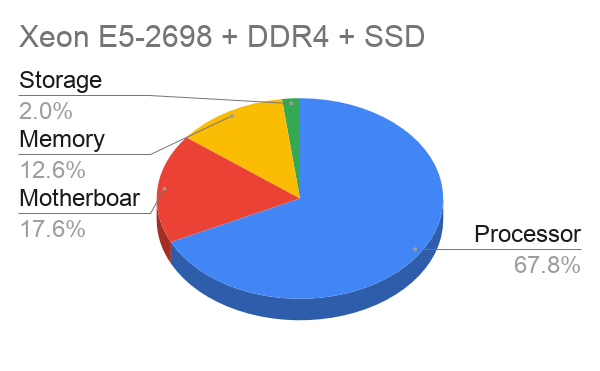
\includegraphics[width=\textwidth]{power_breakdown/Xeon E5-2698 + DDR4 + SSD.png}
    \caption{This work.}
    \label{fig:1}
    \end{subfigure}
    %
    \begin{subfigure}[b]{0.45\textwidth}
    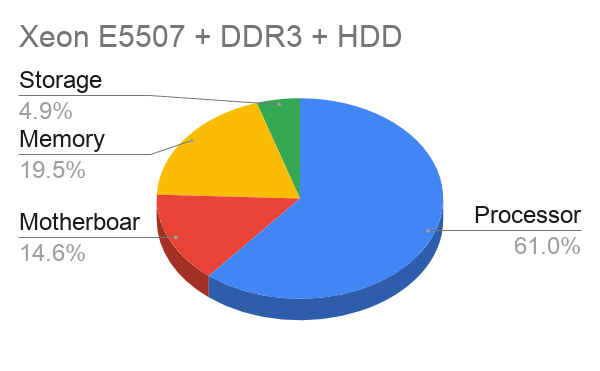
\includegraphics[width=\textwidth]{power_breakdown/Xeon E5507 + DDR3 + HDD.png}
    \caption{Study case in \cite{Malladi2012TowardsDRAM}.}
    \label{fig:2}
    \end{subfigure}
    
    \hfill
    \caption{Power breakdown of a typical node of an HPC cluster at full use. The system used in this work (a) was built in 2016 and equipped with two Intel Xeon E5-2698, 128 GB of DDR4 memory and SSD as storage, while (b) the case study in \cite{Malladi2012TowardsDRAM} was built in 2012 and equipped with two Xeon E5507, 32GB of DDR3 memory and HDD as storage.}
    \label{fig:powerbreakdown}
\end{figure}

DVFS is motivated by the well-known fact that frequency and power have a near-cubic relationship \cite{Dayarathna2016DataSurvey, Group2012HandbookSahni}. 
This implies that running the CPU at lower frequency causes a linear reduction in the performance while a near-cubic reduction in power and, consequently, could lead to a near-square reduction in CPU energy. 
This can lead to dramatic energy savings depending on the system and its architecture.
Although very promising, the system software has yet to determine when and what voltage and frequency to use when running applications.
Otherwise, not only will performance deteriorate, but in the worst case, energy consumption would also increase  \cite{Group2012HandbookSahni}.
Indeed, reducing the frequency results in a longer execution time, which increases the energy consumption of other system components such as memory and disks.
There is also an overhead of time and energy associated with a voltage and frequency switch.
Thus, finding the most appropriate voltage and frequency to use  in all circumstances is not an easy task.
Therefore, since its introduction in 1994, there has been a tremendous amount of research on DVFS algorithms.

The DPM technique can achieve substantial energy savings on systems where the static power is high, or the system remains inactive for a long time.
In that case, the problem is to determine when and which components to turn on/off.
With DPM, energy savings of 70\% have been reported ~\cite{Shuja2012Energy-efficientCenters, Benini2000AManagement}.
%In the case of DPM, the problem is determining when and which components to turn on/off. This technique can achieve substantial energy savings on systems where the static power consumption is high or if the system stays idle for a long time. Power savings of 70\% have been reported~\cite{Shuja2012Energy-efficientCenters, Benini2000AManagement}.

At the same time as the stated techniques reduce the system's energy consumption, they also lead to a complex performance trade-off that must be exploited to produce energy-efficient algorithms.
%However, at the same time, that these power-saving techniques reduce system energy, they also lead to a complex balance between energy savings and high performance, exposing trade-offs between performance and power consumption, which can be exploited to produce more energy-efficient algorithms.  %in the case of the CPU, this can be applied to each core. Here... 
Indeed, this work investigates whether the construction of a model of the energy consumption of an application can lead to significant energy savings. We propose an analytical energy model of an application in function of the two control variables present in most HPC systems: CPU operating frequency and number of active cores. 
%%This model can serve as a base for new DVFS and DPM algorithms as well as for analyzing the contribution of individual model parameters to the total energy consumption.
This model, which characterizes an application, contributes to the objectives of DVFS and DPM techniques since it serves to the analysis of the contribution of each of the parameters to the total energy consumption.
Thus, the model includes two application-dependent parameters and three parameters relating to the system. The application parameters incorporate characteristics of the percentage of parallelism and the size of the input. The system parameters include power-related and technology-dependent components that compose dynamic, static, and leakage power.

The rest of this paper is organized as follows. In Sections \ref{sec:background} and \ref{sec:relatedwork}, a general review of existing models is provided, showing the difference between each approach and its applications. In Section \ref{sec:models}, the proposed model and its parameters are derived alongside its constraints. In Section \ref{sec:experimentalvalidation}, the model is validated with the PARSEC benchmark applications. Forward, in Section \ref{sec:dvfs_optmin}, use cases of the model are presented as well as how it could be applied in DVFS. Finally, the conclusion is made in Section \ref{sec:conclusion}.
 
%%%%%%%%%%%%%%%%%%%%%%%%%%%%%%%%%%%%%%%%%%
\section{Theoretical background} \label{sec:background}

A model is a formal representation of a real system. Computer system models can be represented in the form of equations, graphical models, rules, decision trees, representative collections of examples, or by neural networks, among others. The choice of representation affects the model's accuracy, as well as its interpretability by people~\cite{Hypothesis2012EncyclopediaLearning, Roy2019ForecastingNetwork, Zhu2019PredictingLearning}. Accurate energy and power consumption models are very important for many energy efficiency schemes employed in computing equipment \cite{Rivoire2007ModelsOptimizations}, and they can have multiple uses, including the design, forecasting, and optimization of data center systems. This work focuses on analytical models that could serve for energy optimization and subsequently, analysis of important factors in the total energy draw.

The desirable properties of a full-system model of energy consumption include accuracy (precision enough to allow the required energy saving), speed (fast enough to produce predictions), generality and portability (should be suitable for as many systems as possible), inexpensiveness (should not require costly or invasive infrastructure), and simplicity \cite{Rivoire2008AModels}. However, modeling the exact energy consumption behavior of an HPC system is not straightforward, either at the whole-system level or at the level of individual components. Patterns of energy consumption in data centers depend on multiple factors such as hardware specifications, workload, cooling requirements, or types of applications. Some of these factors cannot be measured easily. Furthermore, it is impractical to perform detailed measurements of the energy consumption of lower-level components without impacting the system with additional overload.

The concept of energy (E) is the total amount of work performed by a system over a period of time (T), while power (P) is the rate at which the system performs the work. The relation between these three amounts can be expressed as:

\begin{equation}
    E = \int_{0}^{T}P(t)dt
    \label{qe:energy_definition_cont}
\end{equation}

Several proposed models have already been classified with respect to its input parameters in \cite{Dayarathna2016DataSurvey}. In this survey, more than 200 models were analyzed according to their characteristics and limitations and classified into categories where the model is more suited to its objectives:
\begin{itemize}
    \item Temperature
    \item System Utilization or Workload
    \item Frequency
    \item Other system states such as cache miss, branch prediction, number of instructions executed, and more
    \label{tab:input_type}
\end{itemize}

Often, energy models are described as a combination of two main parts, the power model of the system and the performance model of the application. 

\subsection{Power models}
Temperature-based models\cite{ZhangEnergyInfrastructure} can provide a way of estimating power consumption without being very intrusive. With this kind of model, it is possible to estimate energy with a single temperature sensor without the need to restart or introduce anything to the system. This is especially interesting for HPCs and data centers which, can not be easily turned off. Another use of this model is in the optimization of the refrigeration systems.

A large part of the developed models are based on parameters representing the state of the system. They normally take advantage of performance counters, which are provided by the CPU or the operating system and are capable of counting micro-architectural events, such as instructions executed, cache-hits, miss-predicted branches, and much more. 
This type of model is suitable for power estimation because it receives information about several internal states of the computer.

Frequency-based models serve as a base for many power models ~\cite{Sarwar1997, Butzen2007, Usman2013ANoC} because at a very low level every digital circuit (including modern processors) is composed of transistors. In these devices, there is a known relationship between power and frequency, which can be simplified by \cref{eq:power_simplified}: 
\begin{equation}
    P = \alpha+\beta f^3
    \label{eq:power_simplified}
\end{equation}
where $\alpha$ and $\beta$ are model parameters, and $f$ is the operating frequency (details of this equation are covered in Section~\ref{sec:models}). These types of models are suitable for optimization problems since they are a function of the operating frequency, which can be easily controlled.

\subsection{Performance models}
Another commonly used way to model the energy consumption of the system is the workload. The workload, which represents the amount of work done in a given time and speed, abstractly defines the application.  

The workload ($W$) can be defined as~\cite{Paolillo2018OptimisationParallelism, Group2012HandbookSahni, Kim2015RacingHeuristics}:
\begin{equation}
    W = \int_{0}^{\tau}s(t)dt = s\tau
    \label{eq:workload_definition}
\end{equation}
where $\tau$ is total active time, and $s$ is the execution speed in instructions/second.
This equation is often taken up by utilization-based models, so that it could be applied to real systems. 

Utilization can be defined as the ratio between the time that the system is active and the total time. Equation (\ref{eq:workload_utilization_tranlation}) defines workload in terms of CPU utilization ($u$):
\begin{equation}
    u = \frac{\tau}{T} = \frac{W/s}{T},
    \label{eq:utilization_definition}
\end{equation}
\begin{equation}
    W = usT,
    \label{eq:workload_utilization_tranlation}
\end{equation}
where $T$ the total execution time of the workload, and $s$ the execution speed.
Models based on CPU utilization are the base for DVFS algorithms. Even though the input is not controllable, it is straightforward  to measure system utilization with almost no overhead, and it is also very portable in terms of operating systems and architectures. 
%% Here is how to build the model or to optimize it, maybe too early to talk about AI without referencing existing approaches:
%There is no need for data and training, as with artificial intelligence algorithms, and adapts reasonably well to any machine. 
A downside is that optimization requires the knowledge of a wide variety of workloads which must be estimated somehow \cite{Fu2018RaceMinimization, Group2012HandbookSahni}.


% Markov model
Other approaches are also adopted to model energy, as for example in the work of Liu et al. \cite{Liu2016IntelligentSupplies} where the model uses a Markov chain to determine energy state transitions. This kind of approach needs heuristic algorithms to search for the best transitions and does not provide insights as an analytical equation does.

Although much work has been done in DVFS, the focus is still on the consumer electronics and laptop markets. 
For HPC, the notion of energy perception is relatively new~\cite{Beckman2005MakingSupercomputing}. 
Moreover, the operational characteristics of non-HPC and HPC systems are significantly different. 
First, the workload on non-HPC systems is very interactive with the end-user, but the workload on the HPC platform is not. 
Second, activities conducted on a non-HPC platform tend to share more machine resources.
In contrast, in HPC each job often runs with dedicated resources. 
Third, an HPC system usually is much larger than non-HPC systems, making it more  challenging to gather information, organize decisions, and execute global decisions.
Therefore, it is worthwhile to investigate whether a DVFS scheduling algorithm, which works well for conventional computing, remains effective for HPC.

\section{Related work} \label{sec:relatedwork}

Merkel et al.~\cite{Merkel2006BalancingSystems} developed an energy model for processors based on events. By counting a set of $n$ events and assuming that the processor consumes a fixed amount of energy $\alpha_i$ for each activity, they estimate the energy in a particular period as the number of occurrences $c_i$  multiplied by its correspondent weight $\alpha_i$:
\begin{equation}
    E = \sum_{i=1}^{n}\alpha_ic_i.
\end{equation}

Another event-based model introduced by Roy et al. \cite{Roy2013AnAlgorithms}, described the computational energy consumed by a CPU for an algorithm $A$:
\begin{equation}
    E(A) = P_{clk}T(A) + P_wW(A),
\end{equation}
where $P_{clk}$ is a processor clock leakage power, $T(A)$ is the total execution time, $W(A)$ is the total time taken by  non-I/O operations, and $P_w$ is used to capture the power consumption per operation performed by the CPU. $T(A)$ and $W(A)$ are estimated using performance features.

Models based on events are implemented using performance counters \cite{Fahad2019AComputing}, which have some drawbacks. They are highly dependent on the operating system and its architecture, making them not so easily portable. Additionally, there are limitations on the number of counters that can be read simultaneously. Furthermore, reading too many counters can add a non-negligible overhead. Thus, modern CPUs start to multiplex counters when more than a few are requested. There are also some well know problems regarding the precision of some events \cite{Weaver2008, Weaver2013a, Das2019SoK:Security, McGuire2009, Ramos2019AnCounters, Silva-De-Souza2020Containergy-aWorkloads}. Events that should be exact and deterministic (such as the number of executed instructions) show run-to-run variations and over-count on x86\_64 machines, even when running in strictly controlled environments. Our proposal is not based on performance counters and, therefore, is not vulnerable to those drawbacks.


Instruction-level energy model was also proposed in \cite{Characterization2013EnergyProcessor}, obtained from an energy per instruction (EPI) characterization made on Xeon Phi. Their model is expressed as:
\begin{equation}
    E(f) = \frac{(p_1 - p_0)(c_1 - c_0)/f}{N}, 
\end{equation}
where $N$ is the total number of dynamic instructions, $p_0$ is the initial idle power, $p_1$ is the average dynamic power and ($c_1$-$c_0$) refers to the cumulative number of cycles the micro-benchmark performs. This model is suitable for estimating the energy after the application finishes executing, when it is possible to count the number of total cycles. However, it is challenging to use for optimization or forecasting since it does not have an application model to predict the number of cycles. Our model integrates the behavior of the application taking into account the execution time.

In \cite{Lewis2008Run-timeSystems} Lewis et al. described the overall system energy consumption using the following equation:
\begin{equation}
E = A_0(E_{proc} + E_{mem}) + A_1E_{em} + A_2E_{board} + A_3E_{hdd},    
\end{equation}
where, $A_0$, $A_1$, $A_2$, and $A_3$ are unknown constants that are calculated via linear regression analysis and those remain constant for a specific server architecture. This model, as the previous one, relies on knowledge of energy spent on each component, being  a suitable option for estimation after the application has already ran, but not for optimization of the run itself.

In another energy consumption model  based on system utilization, Mills et al. modeled the energy consumed by a compute node with CPU (single) executing at speed $\sigma$ as \cite{Mills2014EnergySystems},
\begin{equation}
    E(\sigma,[t_1,t_2]) = \int_{t_1}^{t_2} \sigma^3 + \rho \sigma_max^3 dt,
\end{equation}

where $\rho$ stands for the overhead power  consumed regardless the processor speed, $t_1$ and $t_2$ are the initial and final execution time of the application. The overhead includes power consumption by all other system components such as memory, network, etc. For this reason, although the authors mentioned the energy consumption of a socket, their power model is generalized to the entire server.

Our work proposes a full-system energy model based on the CPU frequency and the number of cores.
The aim of the model is to understand and optimize the energy behavior of parallel applications in HPC systems according to application parameters such as the degree of parallelism and CPU parameters related to dynamic and static power. The proposed model differs from existing ones for including the frequency and number of cores in the same equation for estimating the energy for a specific application in a given configuration. This model can serve as a base for DVFS and DPM optimization problems that include frequency and number of active cores. It can also be used to analyze the contribution of each parameter (ex: level of parallelism) to energy consumption. The number of cores is an essential factor in HPC since applications are designed to run on multiple cores.

The proposed energy model is the product of an application-agnostic power model and an architecture-specific application performance model. The power model is based on the CMOS logic gates power draw as a function of the frequency~\cite{Sarwar1997, Butzen2007} augmented to include the number of cores. The performance model is based on Amdahl's law \cite{Amdahl1967ValidityCapabilities, Eyerman2010ModelingDesign, Shi2015ReevaluatingLaw}, which can be used to estimate runtime in multi-core systems. This model has been extended to include execution frequency and input size, characterizing the application on the target architecture.

%%%%%%%%%%%%%%%%%%%%%%%%%%%%%%%%%%%%%%%%%%

\section{Modeling energy with performance and power} \label{sec:models}
In this section, the three models proposed for power, performance and energy are described.

\subsection{Power Model} \label{sec:powermodel}
The complexity of the modern processor's circuits makes it very difficult to consider all the components and interconnections. A viable approach for modeling the CPU's power draw is to model their building components, mainly made out of logic gates. Thus, modeling the power consumption can be resumed to model the logic gates and multiplying this by the total number of gates, reducing the complexity of the modeling process.

The mature technology to manufacture logic gates is CMOS. Nowadays, it has been replaced by FINFET. In general, in these technologies, there are three main components of power dissipation \cite{Rauber2014, Goel2016, Du2017, Gonzalez1997},  namely, static power $P_{\rm static}$, dynamic power $P_{\rm dynamic}$, and leakage power $P_{\rm leak}$, that accumulated compose the total power draw.
% \begin{equation}
% P=P_{\rm static}+P_{\rm leak}+P_{\rm dynamic}.
% \label{eq:power_breakdown}
% \end{equation}

The dynamic power and leakage power behavior can be approximated by \cref{eq:power_dyn} and \cref{eq:power_leak}, respectively, as shown by Sarwar et al. and Butzen et al~\cite{Sarwar1997, Butzen2007}.
\begin{equation}
P_{dynamic}=CV^2f,
\label{eq:power_dyn}
\end{equation}
\begin{equation}
P_{leak} \propto V,
\label{eq:power_leak}
\end{equation}
where $C$ is the load capacitance, $V$ the voltage applied to the circuit and $f$ the switching frequency.

Another common approximation is to expect a linear relationship between the voltage and the applied frequency~\cite{Usman2013ANoC} such that:
\begin{equation}
f \propto V,
\label{eq:f_v}
\end{equation}
Thus, the proposed model for one processing core of a multi-core processor is derived by using \cref{eq:power_dyn}, \cref{eq:power_leak} and \cref{eq:f_v} to write \cref{eq:total_power}.
\begin{equation}
P(f)= c_1f^3+c_2f+c_3,
\label{eq:total_power}
\end{equation}
where $c_1$ $c_2$, and $c_3$ are the model's parameters associated with the dynamic, leakage and static power aspects, respectively. Including the number of active cores $p$, the proposed estimation of the power consumption of the whole processor becomes \cref{eq:power_final}
\begin{equation}
P(f,p)= p(c_1f^3+c_2f)+c_3,
\label{eq:power_final}
\end{equation}

\subsection{Performance Model} \label{sec:performancemodel}
To model the application execution time, we consider a program as a set of instructions executed on a mean frequency $f$ with $c_k$ instructions per cycle. The time $T_f$ that this program will take to complete at a given frequency is devised as follows:
\begin{equation}
T_f=\frac{I}{c_kf},
\label{eq:freqrel}
\end{equation}
where $I$ is the total number of instructions and $c_k$ the ratio of instructions per unit of time.

The next step is to include the number of cores in the equation. Amdahl's law \cite{Amdahl1967ValidityCapabilities}, described in \cref{eq:amdahl}, gives the theoretical background for that. It describes the speedup in latency of the execution of a task at a fixed workload.
\begin{equation}
S=\frac{T_s}{T_p}=\frac{1}{1-w+\frac{w}{p}},
\label{eq:amdahl}
\end{equation}
where $T_s$ is the serial time, $T_p$ the parallel time, $S$ is the theoretical speedup of the execution of the whole task, $w$ is the proportion of the execution time that benefits from improving system resources, and $p$ is the part of the task that benefits from improved system resources. Combining this with \cref{eq:freqrel}, the parallel time at frequency $f$ can be written as:
\begin{equation}
T_p=\frac{T_s}{S}=\frac{T_f}{\frac{1}{1-w+\frac{w}{p}}},
\label{eq:parallel_time}
\end{equation}

We can then write the equation of the program execution time as a function of frequency, number of cores and parallelism  as \cref{eq:performance} and subsequently derive \cref{eq:performance_2}:
\begin{equation}
T(f,p)=\frac{I}{ \frac{c_kf}{1-w+\frac{w}{p}} },
\label{eq:performance}
\end{equation}
\begin{equation}
T(f,p)=\frac{d_1(p-wp+w)}{fp},
\label{eq:performance_2}
\end{equation}
where $d_1$ is a constant.

Finally, to fully characterize the application, a parameter representing the application's workload, called input size $N$, is introduced, representing the number of basic operations need to complete a problem \cite{Kumar1994AnalyzingArchitectures}. In Oliveira et al. \cite{Oliveira2018ApplicationCores}, they showed that this parameter could generally be described as exponential. Therefore the proposed performance model is presented in \cref{eq:performance_final}. This resulting equation can describe the behavior of the execution time of a program for an input $N$, frequency $f$, and active cores $p$:
\begin{equation}
T(f,p,N)=\frac{d_1N^{d_2}(p-wp+w)}{fp},
\label{eq:performance_final}
\end{equation}
where $d_1$, $d_2$ and $w$ are constants that depend on the application. 

\subsection{Energy Model} \label{sec:energymodel}
Combining the power model output described in~\cref{sec:powermodel} and the characterization of the application performance described in \cref{sec:performancemodel}, the total energy can be modeled as:
\begin{equation}
E(f,p,N)=P(f,p)\times{\rm T}(f,p,N),
\label{eq:en_combination}
\end{equation}
where $P(f,p)$ is the total power modeled by~\cref{eq:power_final}, ${T}(f,p,N)$ is the execution time estimated by the \cref{eq:performance_final}, $f$ is the frequency, $p$ is the number of active cores, and $N$ is the input size. The final equation can be written as:
\begin{equation}
    E(f,p,N)=\frac{d_1N^{d_2}(p-wp+w)(p(c_1f^3+c_2f)+c_3)}{fp}.
    \label{eq:en_final}
\end{equation}

%%%%%%%%%%%%%%%%%%%%%%%%%%%%%%%%%%%%%%%%%%

\section{Experimental validation} \label{sec:experimentalvalidation}
In this section, the models presented in~\cref{sec:powermodel} and~\cref{sec:performancemodel} were validated with a benchmark specific for multi-core architectures. Additionally, in order to assess the modeling overhead and accuracy, our proposal was then compared to machine learning approaches. We compared against Support Vector Regression (SVR)~\cite{Smola2004}, Decision Tree \cite{Kitts2006RegressionLecture}, k-nearest neighbors \cite{Altman1992AnRegression}, Multilayer perceptron \cite{Murtagh1991MultilayerRegression}, and some new methods such as Gao et al. \cite{Gao2019DendriticPrediction}. However, SVR was chosen as the most representative because in our tests it performed best without an aggressive fine-tuning.

\subsection{Case-Study Applications} \label{sec:casestudyapplication}
The PARSEC parallel benchmark suite, version 3.0~\cite{Bienia2008}, OpenMC \cite{Romano2015OpenMC:Development} and LINPACK (HPL) \cite{Dongarra1988TheExplanation}, were chosen as case studies. The PARSEC benchmark focused on emerging workloads and was designed to represent the next-generation shared-memory programs for chip-multiprocessors. It covers an ample range of areas such as financial analysis, computer vision, engineering, enterprise storage, animation, similarity search, data mining, machine learning, and media processing. The OpenMC and the LINPACK are two classic HPC programs.

\subsection{Case-Study Architecture} \label{sec:casestudyarchitecture}
The experiments were executed in one computer node equipped with two Intel Xeon E5-2698 v3 processors with sixteen cores each and two hardware threads for each core. The overall view of the architecture is shown in Figure \ref{fig:architecture}. The maximum non-turbo frequency is 2.3GHz, and the total physical memory of the node is 128GB (8$\times$16GB). Turbo frequency and hardware multi-threading were disabled during all experiments. The operating system used was Linux CentOS 6.5, kernel 4.16. 

\begin{figure}[htb!]
    \centering
    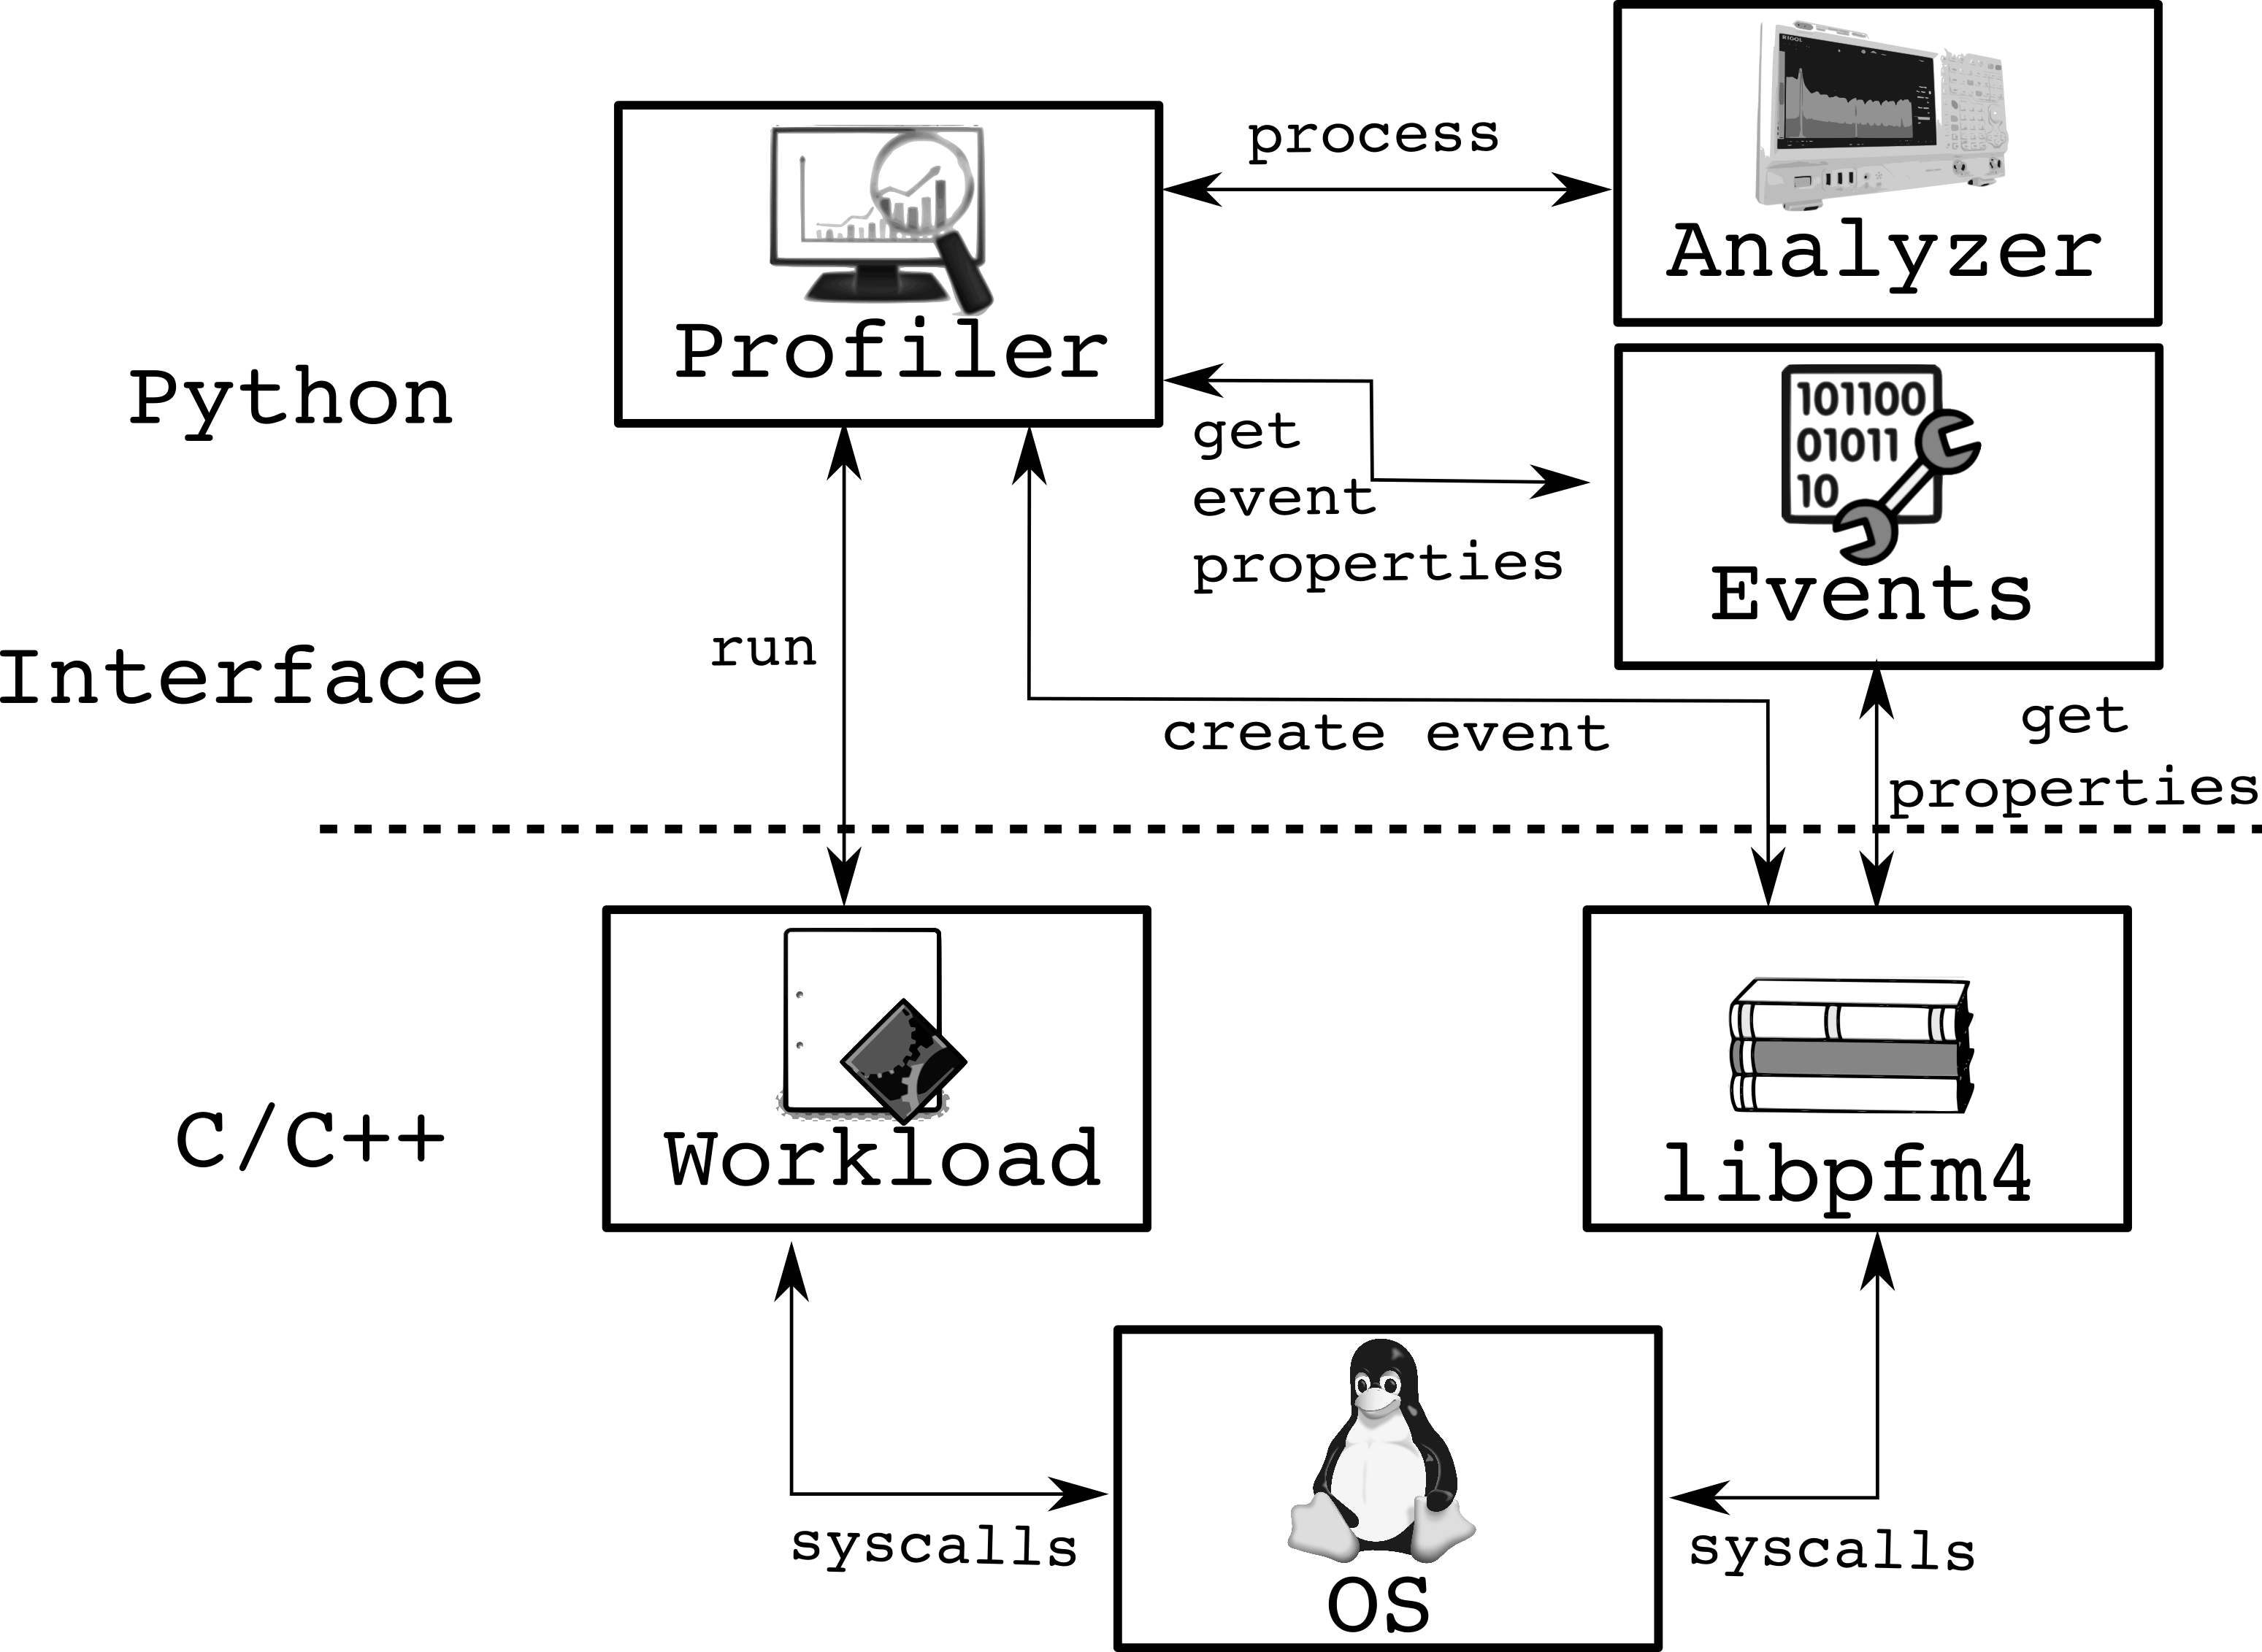
\includegraphics[width=\columnwidth]{architecture.png}
    \caption{Node architecture (the image was made with the lstop application).}
    \label{fig:architecture}
\end{figure}

The Linux kernel has many different policies for power management, depending on the driver. In the default driver, the acpi-cpufreq, the options are:
\begin{itemize}
    \item Powersave
    \item Performance
    \item Ondemand
    \item Conservative
    \item Userspace
\end{itemize}
In this work, the frequency control was performed using the Userspace governor, and the core control was accomplished by modifying the appropriate system files with the default CPU-hotplug driver.

The architecture is equipped with the Intelligent Platform Management Interface (IPMI), a set of interfaces allowing out-of-band management of computer systems and platform-status monitoring via the local network~\cite{Schwenkler2006IntelligentInterface}. It can monitor variables and resources such as the system's temperature, voltage, fans, and power supplies, with independent sensors attached to the hardware.

\subsection{Fitting the Models} \label{sec:fitting}
To find the parameters of the \cref{eq:en_final}, 10 uniformly random configurations of frequencies ($f$), cores ($p$) and inputs ($N$) were chosen from the range $1<=p<=32$, $1.2<=f<=2.2$ and $1<=N<=5$ respectively. The application was executed for each chosen configuration, and the measured  energy and time values were collected. For the input size if we assume that all CPU instructions are executed at approximately the same time, the number of basic operations will be directly correlated with the time. Thus, we can estimate the problem size by looking at the execution time, allowing us to divide a large problem size into several smaller ones knowing their relationship as done in the work of Oliveira ~\cite{Oliveira2018ApplicationCores}. The unity can also vary depending on the definition. In our case for simplicity, we assign numbers from 1 the smallest size to 10 the largest, increasing the problem linearly, that way its also possible to interpolate any input in between these values.

%The application's input was chosen to increase the workload linearly, from smallest to largest, so that most of the input space is covered~\cite{Oliveira2018ApplicationCores}. 

For each configuration, samples of the power were collected using IPMI every 1 second. This sampling rate was chosen because the order of magnitude of the mean run time of the applications is minutes. Therefore, this rate provides enough samples to measure average power. Additionally, timestamps and the total run time were collected. The total energy spent on each configuration is estimated by first interpolation the power samples using a first order method and then integrating this function in the time.

From the sampled data, the parameters of the model can be estimated. This results in an optimization problem of finding the parameters that minimize the distance between estimated and the measured values. To solve this minimization problem, non-linear least squares have been applied. 

The python library scikit-learning was used to build the SVR model~\cite{PedregosaFandVaroquauxGandGramfortAandMichel2011Scikit-learn:Python}. The SVR was trained using the same data used for parameters estimation of \cref{eq:en_final} with a grid search used to find the best kernel function and the best values for the hyper-parameters penalty for the wrong ($C$) and ($\gamma$). For this data, the best function was the Radial Base Function (RBF), and the hyper-parameters were $C=10^4$ and $\gamma=0.5$. 

\subsection{Verifying Hypothesis}
\subsubsection{Frequency and voltage relation}

\begin{figure}[H]
    \centering
    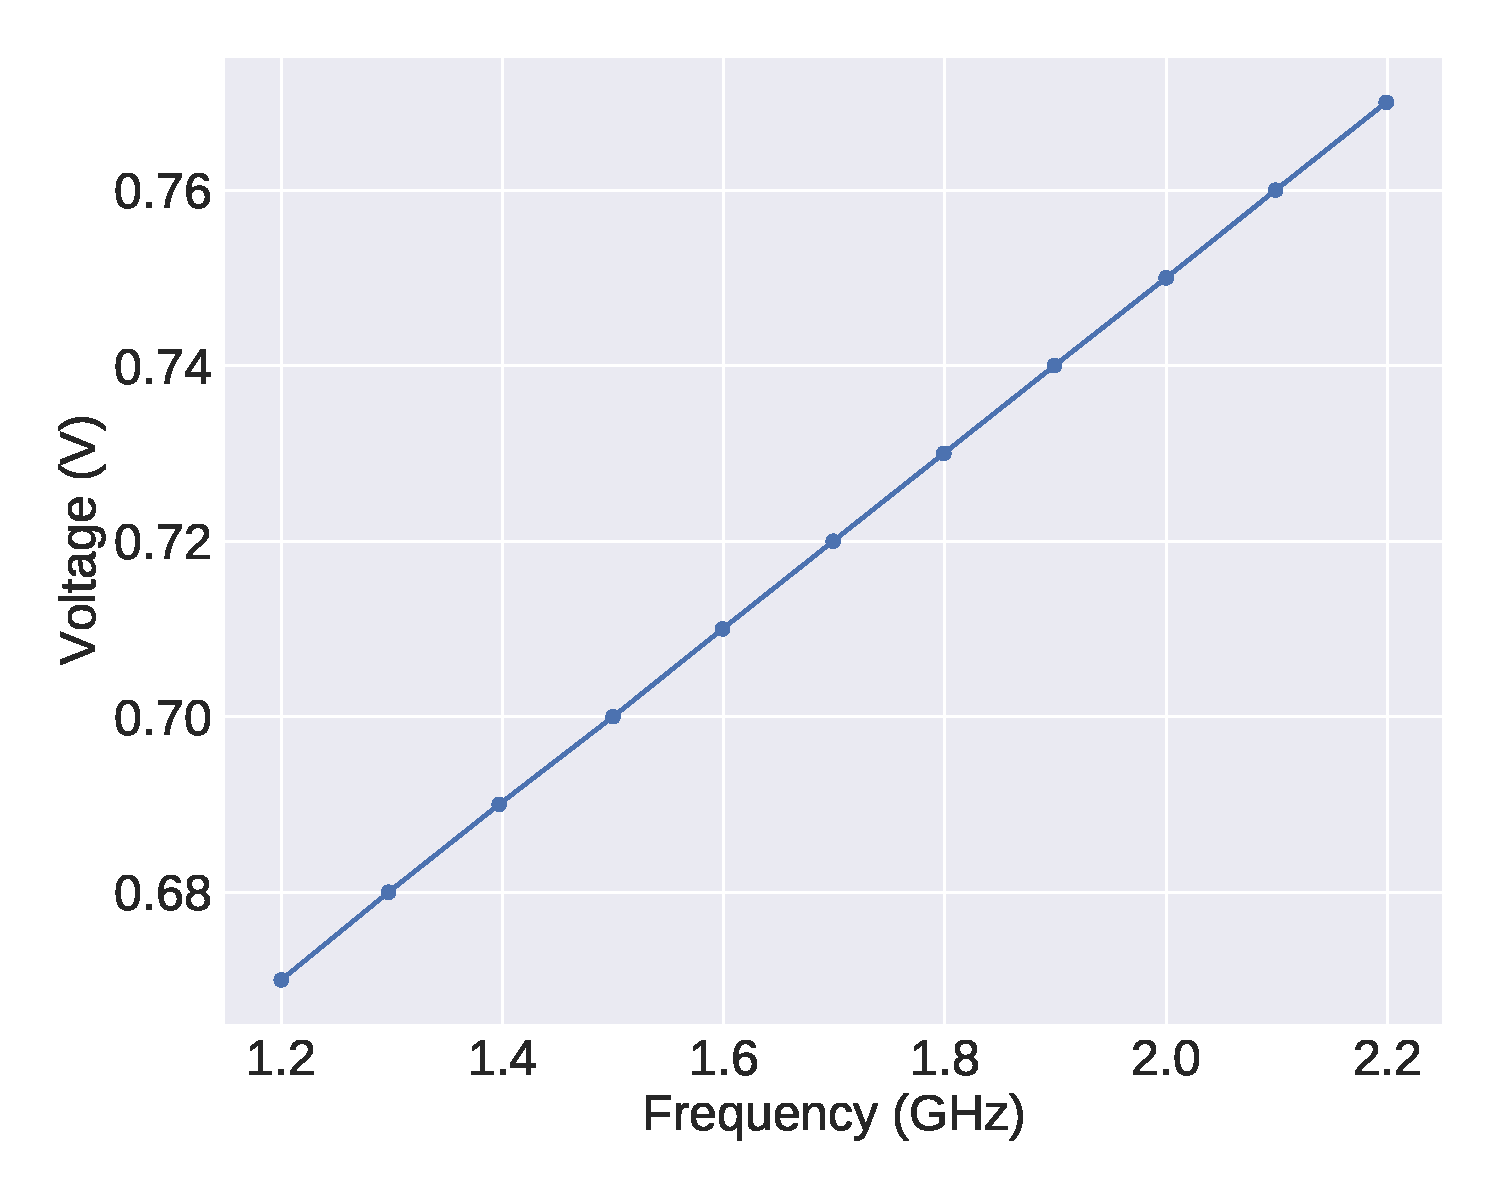
\includegraphics[width=\columnwidth]{hypothesis/freq_volt_rel.png}
    \caption{Frequency voltage relation}
    \label{fig:freq_volt_rel}
\end{figure}

\begin{table}[H]
\caption{Frequency voltage relation}
\centering
\begin{tabular}{|c|c|c|}
\hline
\begin{tabular}[c]{@{}c@{}}Freq. \\ Setted\end{tabular} & Volt. & \begin{tabular}[c]{@{}c@{}}Measured \\ Freq.\end{tabular} \\ \hline
2.2                                                     & 0.77  & 2.199                                                     \\ \hline
2.1                                                     & 0.76  & 2.099                                                     \\ \hline
2.0                                                     & 0.75  & 2.000                                                     \\ \hline
1.9                                                     & 0.74  & 1.899                                                     \\ \hline
1.8                                                     & 0.73  & 1.799                                                     \\ \hline
1.7                                                     & 0.72  & 1.699                                                     \\ \hline
1.6                                                     & 0.71  & 1.599                                                     \\ \hline
1.5                                                     & 0.70  & 1.500                                                     \\ \hline
1.4                                                     & 0.69  & 1.397                                                     \\ \hline
1.3                                                     & 0.68  & 1.297                                                     \\ \hline
1.2                                                     & 0.67  & 1.200                                                     \\ \hline
\end{tabular}
\end{table}

\subsubsection{Instructions executed}

\begin{table}[H]
\caption{Cores variation}
\begin{tabular}{|c|c|c|c|}
\hline
Application  & Instructions & Dev.     & Dev. (\%) \\ \hline
Vip          & 7.97e+11     & 7.16e+06 & 0.00\%    \\ \hline
Openmc       & 8.17e+07     & 1.65e+04 & 0.02\%    \\ \hline
Rtview       & 9.91e+12     & 1.55e+09 & 0.02\%    \\ \hline
X264         & 4.52e+11     & 5.81e+07 & 0.01\%    \\ \hline
Bodytrack    & 1.86e+12     & 3.95e+10 & 2.13\%    \\ \hline
Fluidanimate & 2.09e+12     & 8.44e+10 & 4.04\%    \\ \hline
Xhpl         & 1.14e+08     & 1.24e+05 & 0.11\%    \\ \hline
Blackschole  & 3.75e+12     & 1.40e+09 & 0.04\%    \\ \hline
Dedup        & 1.02e+11     & 5.74e+07 & 0.06\%    \\ \hline
Swapti       & 2.43e+12     & 8.87e+08 & 0.04\%    \\ \hline
Canneal      & 1.19e+11     & 4.46e+07 & 0.04\%    \\ \hline
Freqmine     & 1.27e+12     & 4.78e+08 & 0.04\%    \\ \hline
Ferret       & 4.76e+11     & 7.04e+07 & 0.01\%    \\ \hline
\end{tabular}
\end{table}

\begin{table}[H]
\caption{Frequency Variation}
\begin{tabular}{|c|c|c|c|}
\hline
Application  & Instructions & Dev.     & Dev. (\%) \\ \hline
Vip          & 7.97e+11     & 1.16e+06 & 0.00\%    \\ \hline
Openmc       & 8.17e+07     & 4.52e+03 & 0.01\%    \\ \hline
Rtview       & 9.91e+12     & 6.64e+05 & 0.00\%    \\ \hline
X264         & 4.52e+11     & 1.54e+05 & 0.00\%    \\ \hline
Bodytrack    & 1.84e+12     & 2.54e+05 & 0.00\%    \\ \hline
Fluidanimate & 2.38e+12     & 1.70e+09 & 0.07\%    \\ \hline
Xhpl         & 1.14e+08     & 5.95e+03 & 0.01\%    \\ \hline
Blackschole  & 3.75e+12     & 4.36e+05 & 0.00\%    \\ \hline
Dedup        & 1.02e+11     & 8.32e+07 & 0.08\%    \\ \hline
Swapti       & 2.43e+12     & 1.48e+05 & 0.00\%    \\ \hline
Canneal      & 1.19e+11     & 3.01e+05 & 0.00\%    \\ \hline
Freqmine     & 1.27e+12     & 3.70e+08 & 0.03\%    \\ \hline
Ferret       & 4.76e+11     & 5.63e+07 & 0.01\%    \\ \hline
\end{tabular}
\end{table}

\subsubsection{Input size and instructions}

\begin{figure}[H]
    \centering
    \includegraphics[width=\columnwidth]{hypothesis/input_instructions/fp/Blackschole.png}
    \caption{Caption}
    \label{fig:my_label}
\end{figure}

\begin{figure}[H]
    \centering
    \includegraphics[width=\columnwidth]{hypothesis/input_instructions/fp/Canneal.png}
    \caption{Caption}
    \label{fig:my_label}
\end{figure}

\begin{figure}[H]
    \centering
    \includegraphics[width=\columnwidth]{hypothesis/input_instructions/input_time/Blackschole.png}
    \caption{Caption}
    \label{fig:my_label}
\end{figure}

\begin{figure}[H]
    \centering
    \includegraphics[width=\columnwidth]{hypothesis/input_instructions/input_time/Canneal.png}
    \caption{Caption}
    \label{fig:my_label}
\end{figure}

\subsection{Measured versus Modeled Energy}
\label{sec:measuredversusmodeledenergy}

To validate the proposed energy model, all possible configurations were tested by varying the cores in a range of $1<=p<=32$, the frequency in $1.2<=f<=2.2$ and the input in $1<=N<=5$, which varies from 400 to over 1000 configurations depending on the application as some applications have restrictions on the number of cores. The mean percentage error was computed as the difference between the estimated and measured values according to the following equation:
\begin{equation}
    MPE = \frac{1}{N} \sum_i^N \frac{|y_{\rm estimated}-y_{\rm measured}|}{y_{\rm measured}}.
    \label{eq:mpe}
\end{equation}

\subsubsection{Frequency x Cores}
Figures \ref{fig:en_eq_black}, \ref{fig:en_eq_canneal} plot the measured and modeled energy consumption for some of the applications modeled. They  show some of the possible shapes that the model can take while varying the number of active cores, operating frequency, and input size.
\begin{figure}[H]
    \centering
    \begin{subfigure}[b]{0.48\textwidth}
    	\centerline{\includegraphics[width=\columnwidth]{energy/freq_cores/completo_black_5.png}}
        \caption{Blackscholes.}
    	\label{fig:en_eq_black}
    \end{subfigure}
    %
    \begin{subfigure}[b]{0.48\textwidth}
	\centerline{\includegraphics[width=\columnwidth]{energy/freq_cores/completo_canneal_1.png}}
    \caption{Canneal.}
	\label{fig:en_eq_canneal}
    \end{subfigure}
	\caption{Example fit for a specific input size: Blackscholes (a) and Canneal (b).  “measured values” are the sensor data and “minimum energy” is the minimum energy model prediction.
	}
\end{figure}
\subsubsection{Frequency x Input}
Figures \ref{fig:en_eq_black}, \ref{fig:en_eq_canneal} plot the measured and modeled energy consumption for some of the applications modeled. They  show some of the possible shapes that the model can take while varying the number of active cores, operating frequency, and input size.
\begin{figure}[H]
    \centering
    \begin{subfigure}[b]{0.48\textwidth}
    	\centerline{\includegraphics[width=\columnwidth]{energy/freq_inps/completo_black_5.png}}
        \caption{Blackscholes.}
    	\label{fig:en_eq_black}
    \end{subfigure}
    %
    \begin{subfigure}[b]{0.48\textwidth}
	\centerline{\includegraphics[width=\columnwidth]{energy/freq_inps/completo_canneal_1.png}}
    \caption{Canneal.}
	\label{fig:en_eq_canneal}
    \end{subfigure}
	\caption{Example fit for a specific input size: Blackscholes (a) and Canneal (b).  “measured values” are the sensor data and “minimum energy” is the minimum energy model prediction.
	}
\end{figure}
\subsubsection{Cores x Input}
Figures \ref{fig:en_eq_black}, \ref{fig:en_eq_canneal} plot the measured and modeled energy consumption for some of the applications modeled. They  show some of the possible shapes that the model can take while varying the number of active cores, operating frequency, and input size.
\begin{figure}[H]
    \centering
    \begin{subfigure}[b]{0.48\textwidth}
    	\centerline{\includegraphics[width=\columnwidth]{energy/cores_inps/completo_black_5.png}}
        \caption{Blackscholes.}
    	\label{fig:en_eq_black}
    \end{subfigure}
    %
    \begin{subfigure}[b]{0.48\textwidth}
	\centerline{\includegraphics[width=\columnwidth]{energy/cores_inps/completo_canneal_1.png}}
    \caption{Canneal.}
	\label{fig:en_eq_canneal}
    \end{subfigure}
	\caption{Example fit for a specific input size: Blackscholes (a) and Canneal (b).  “measured values” are the sensor data and “minimum energy” is the minimum energy model prediction.
	}
\end{figure}


\subsubsection{Validation}
The validation results for each application trained with 10 random configurations are displayed in figure \ref{fig:mpe_svr_eq} and the raw MPE values in  table~\ref{tab:mpe_svr_eq}.
\begin{figure}[htb!]
	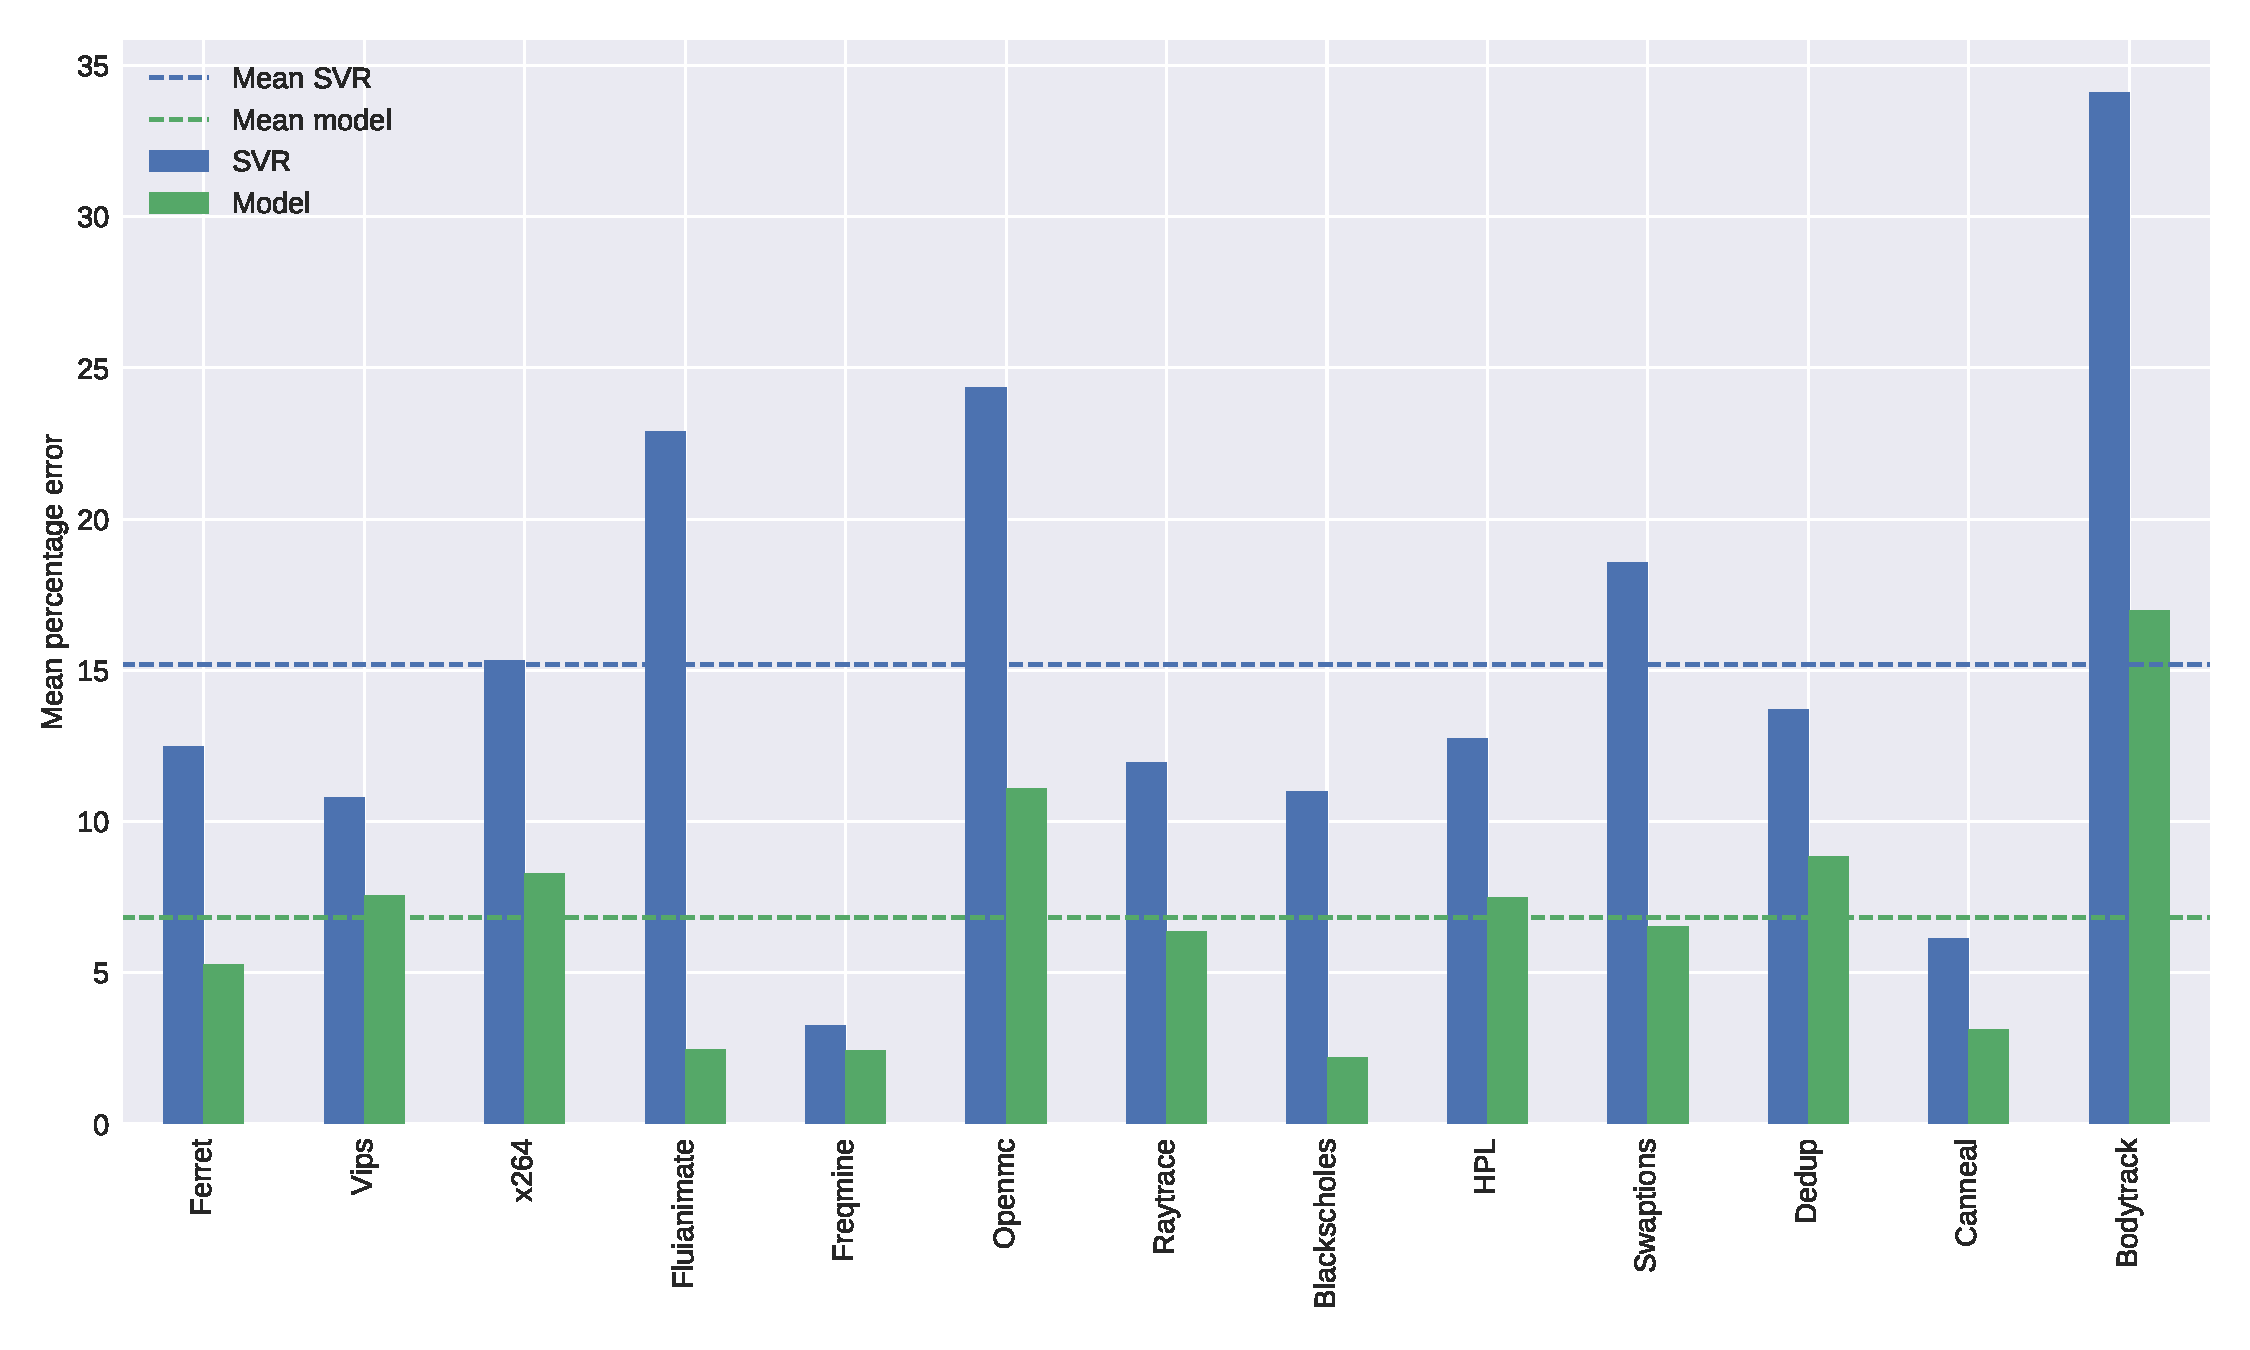
\includegraphics[width=\columnwidth]{mpe_svr_eq.png}
	\caption{Comparison of the Mean Percentage Error between the proposed model and SVR. "Model mean" and "SVR mean" are the average of all MPE values for all applications.
	}
	\label{fig:mpe_svr_eq}
\end{figure}
\begin{table}[htb!]
\centering
\begin{tabular}{|c|c|c|}
\hline
Application  & Model & SVR   \\ \hline
Ferret       & 5.25     & 12.49  \\ \hline
Raytrace     & 6.36     & 11.95  \\ \hline
Fluianimate  & 2.44     & 22.90  \\ \hline
x264         & 8.28     & 15.33  \\ \hline
Vips         & 7.54     & 10.80  \\ \hline
Swaptions    & 6.54     & 18.57  \\ \hline
Canneal      & 3.12     & 6.13   \\ \hline
Dedup        & 8.85     & 13.70  \\ \hline
Freqmine     & 2.44     & 3.24   \\ \hline
Blackscholes & 2.18     & 11.00  \\ \hline
HPL          & 7.47     & 12.75  \\ \hline
Bodytrack    & 16.98    & 34.12  \\ \hline
Openmc       & 11.15    & 24.34  \\ \hline
\end{tabular}
\caption{Comparison of the Mean Percentage Error between the proposed model and SVR: raw values.}
\label{tab:mpe_svr_eq}
\end{table}

Figure \ref{fig:mpe_svr_eq} shows that the proposed model always performed better, with a lower MPE, than SVR when we were limited to 10 training points. This result will be further explored in \cref{sec:overhead} where we compare with different training sizes.

\subsection{Overheads on training} \label{sec:overhead}
It is known that machine learning is data-driven, in that sense the SVR model obtained using only 10 configurations could be improved, but what about the analytical model? 
To answer that question, the proposed model and the SVR were also trained with a varying  number of configurations.
We then compared the MPE and the amount of energy spent to create each model. 
This accuracy-energy trade-off is crucial since the energy overhead when building models defeats the primary goal of saving power when running applications.


\begin{figure}[H]
    \centering
    \begin{subfigure}[b]{0.45\textwidth}
    	\centerline{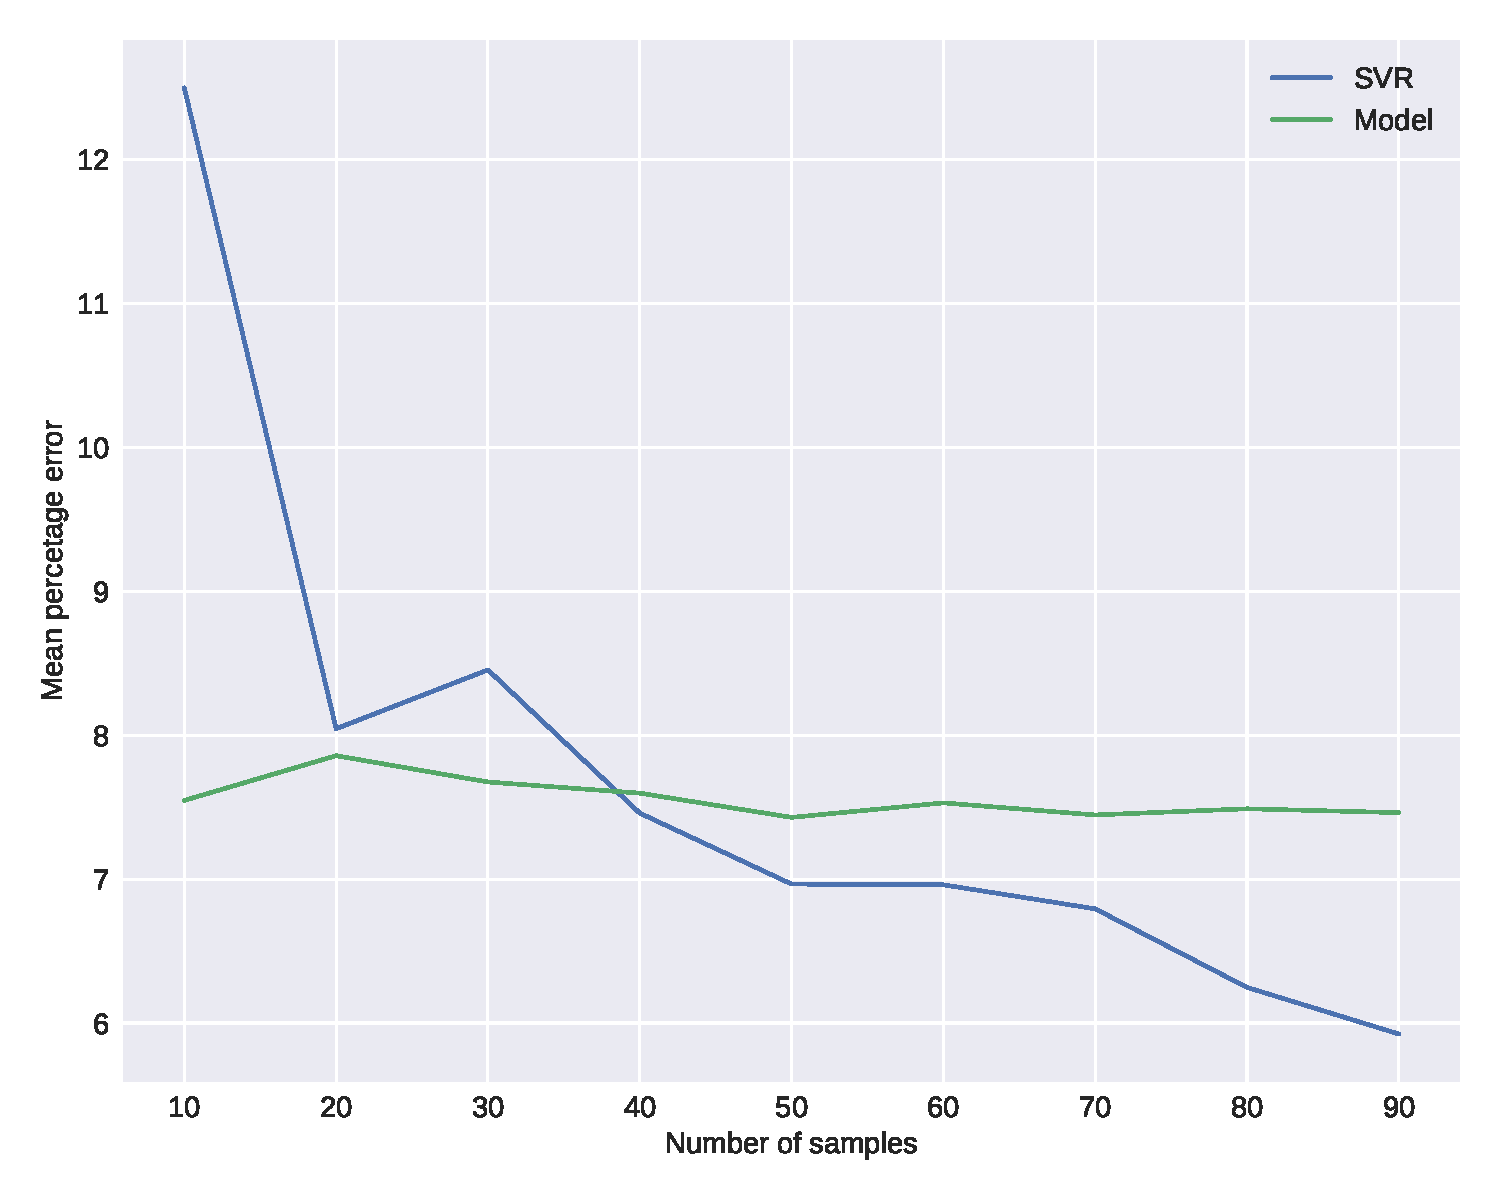
\includegraphics[width=\columnwidth]{overhead/completo_ferret_4.png}}
        \caption{MPE for Ferret.}
    	\label{fig:overhead_ferret}
    \end{subfigure}
    %
    \begin{subfigure}[b]{0.45\textwidth}
    	\centerline{\includegraphics[width=\columnwidth]{overhead/completo_vips_4.png}}
        \caption{MPE for Vips.}
    	\label{fig:overhead_vips}
    \end{subfigure}
    %
    \begin{subfigure}[b]{0.45\textwidth}
    	\centerline{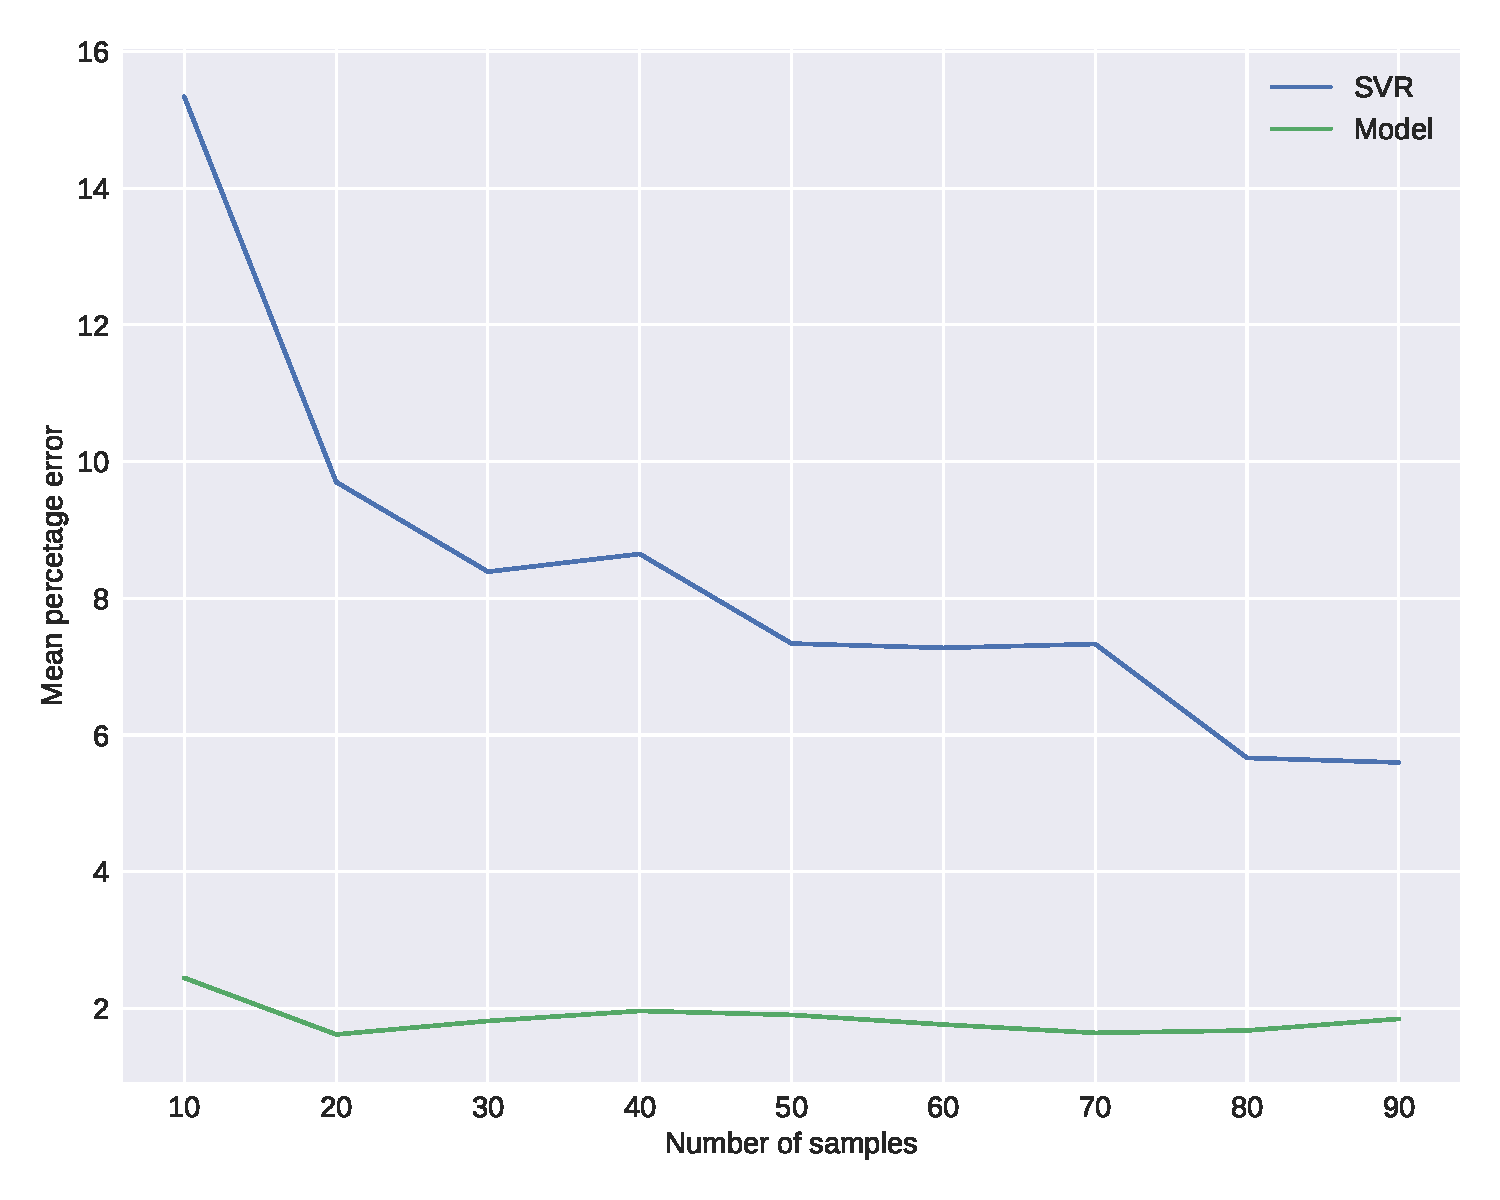
\includegraphics[width=\columnwidth]{overhead/completo_x264_4.png}}
        \caption{MPE for x264.}
    	\label{fig:overhead_x264}
    \end{subfigure}
    \caption{MPE case studies: Ferret (a), Vips (b) and x264 (c): model (almost constant) versus SVR (lowest MPE beyond train-size 35 on case (b)).}
    \label{fig:overheadFerretVips}
\end{figure}

Figure \ref{fig:overheadFerretVips} shows the comparisons of MPE and energy spent to create each model for two selected applications. According to the results, the analytical model is found to be very stable, not changing much as more data is added, while the SVR keeps reshaping to adapt to the data. 
The error of the analytical model is almost constant but that of  the SVR, initially very high, drops at some point.
\begin{figure}[H]
    \centering
    \begin{subfigure}[b]{0.44\textwidth}
    	\centerline{\includegraphics[width=\columnwidth]{overhead/overall.png}}
        \caption{Average energy spent on all applications during model creation. The two curves are identical because the same data were used to adjust the SVR and the model.}
    	\label{fig:overall_overhead}
    \end{subfigure}
    %
    \quad
    \begin{subfigure}[b]{0.44\textwidth}
    	\centerline{\includegraphics[width=\columnwidth]{overhead/overall_mpe.png}}
        \caption{
        MPE all applications: SVR needs 10 times more data to have an MPE lower than the model.}
    	\label{fig:overall_MPE}
    \end{subfigure}
    \caption{Overall results for energy and MPE for each training size.}
    \label{fig:overall_train}
\end{figure}
Figure \ref{fig:overall_train} presents the overall results, with the mean energy overhead and MPE for all applications.
The meeting point of the MPE for the SVR and the proposed model can be extracted from  \ref{fig:overall_MPE}.
There it shows that around 90 configurations the SVR starts to have a smaller error. The cost of that is the linear increase in energy spent on training. The increase in energy, about 10 times more, can be observed in Figure \ref{fig:overall_overhead}.

\subsection{Analysis}

\begin{figure}
    \centering
    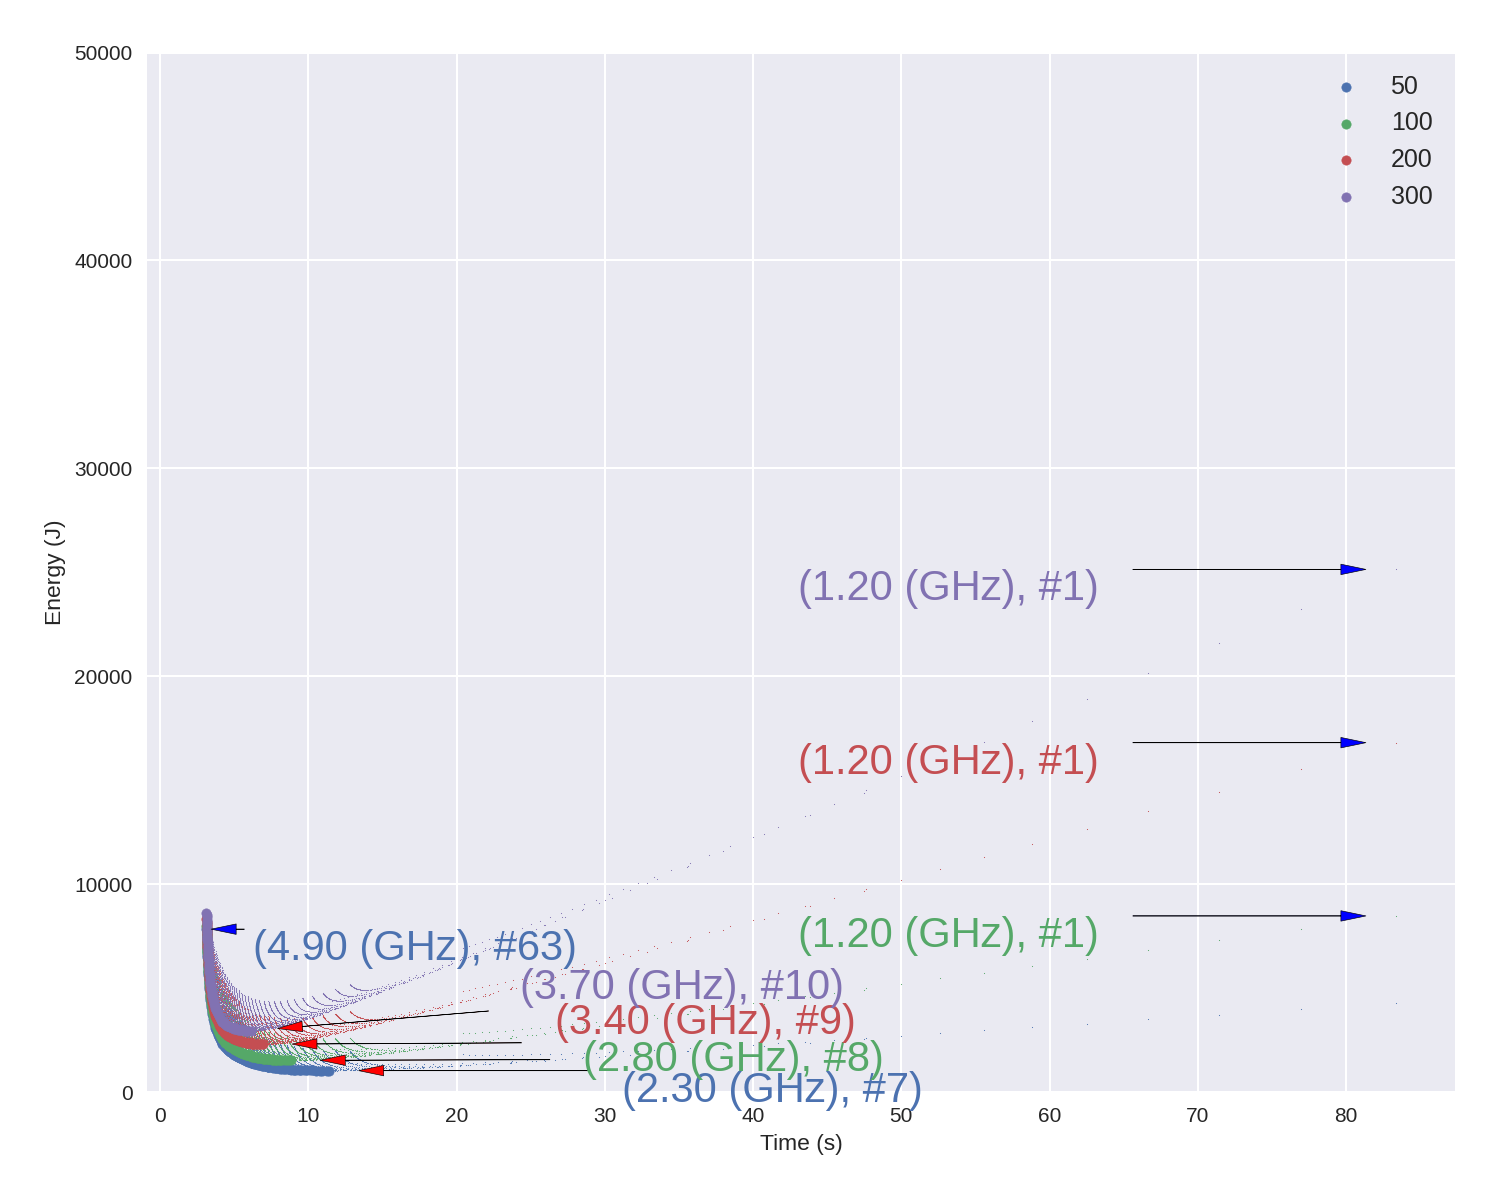
\includegraphics[width=\columnwidth]{analisys/pareto_static_high.png}
    \caption{Pareto static energy}
    \label{fig:pareto_static_h}
\end{figure}


\begin{figure}
    \centering
    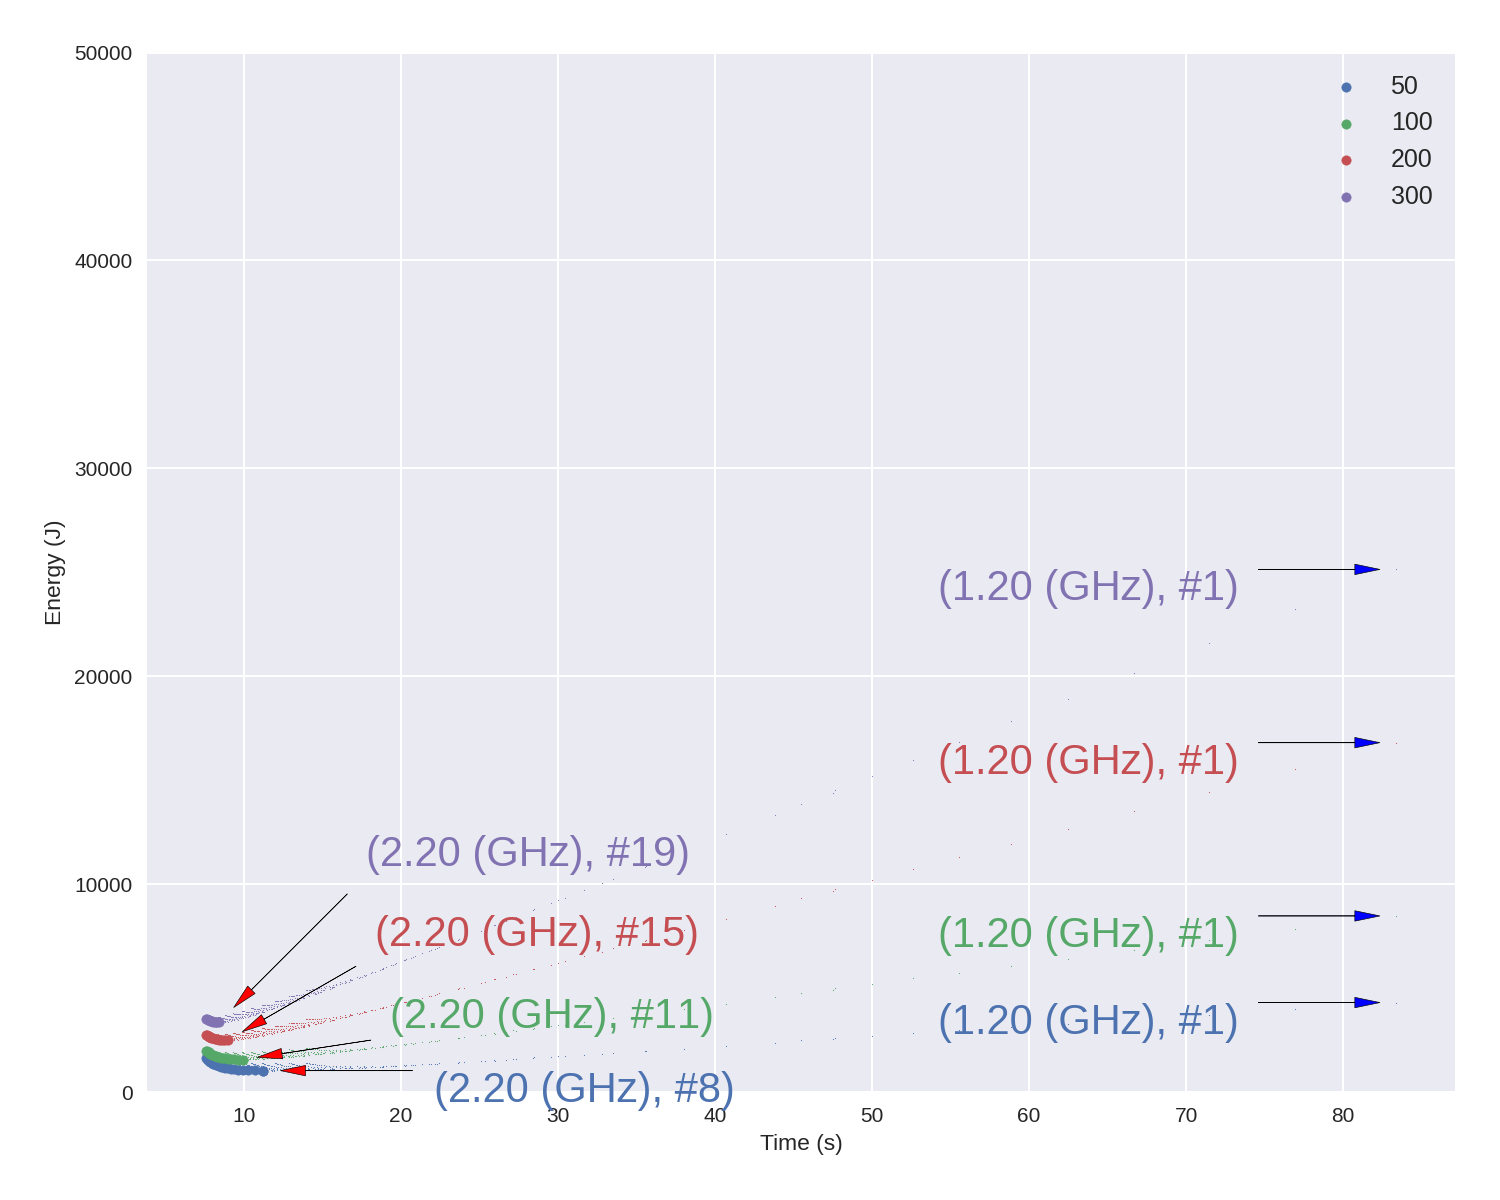
\includegraphics[width=\columnwidth]{analisys/pareto_static_low.png}
    \caption{Pareto static energy}
    \label{fig:pareto_static_l}
\end{figure}


\begin{figure}
    \centering
    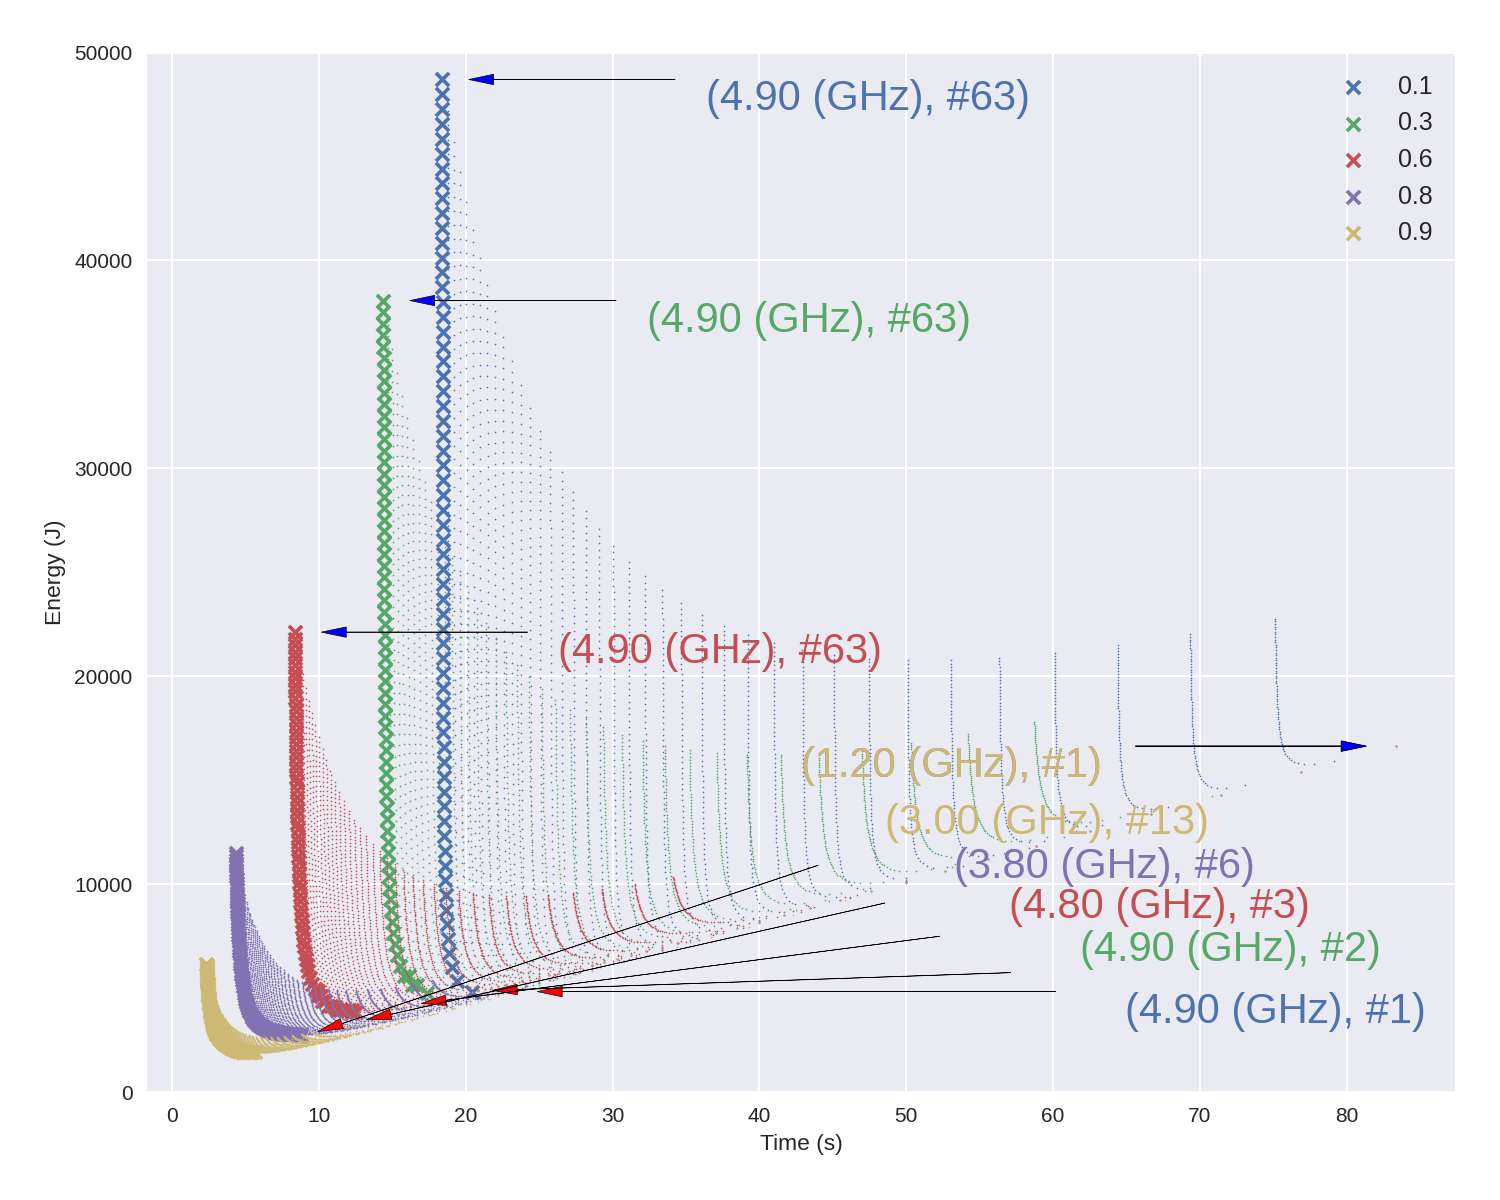
\includegraphics[width=\columnwidth]{analisys/pareto_w_high.png}
    \caption{Pareto w energy}
    \label{fig:pareto_w_h}
\end{figure}

\begin{figure}
    \centering
    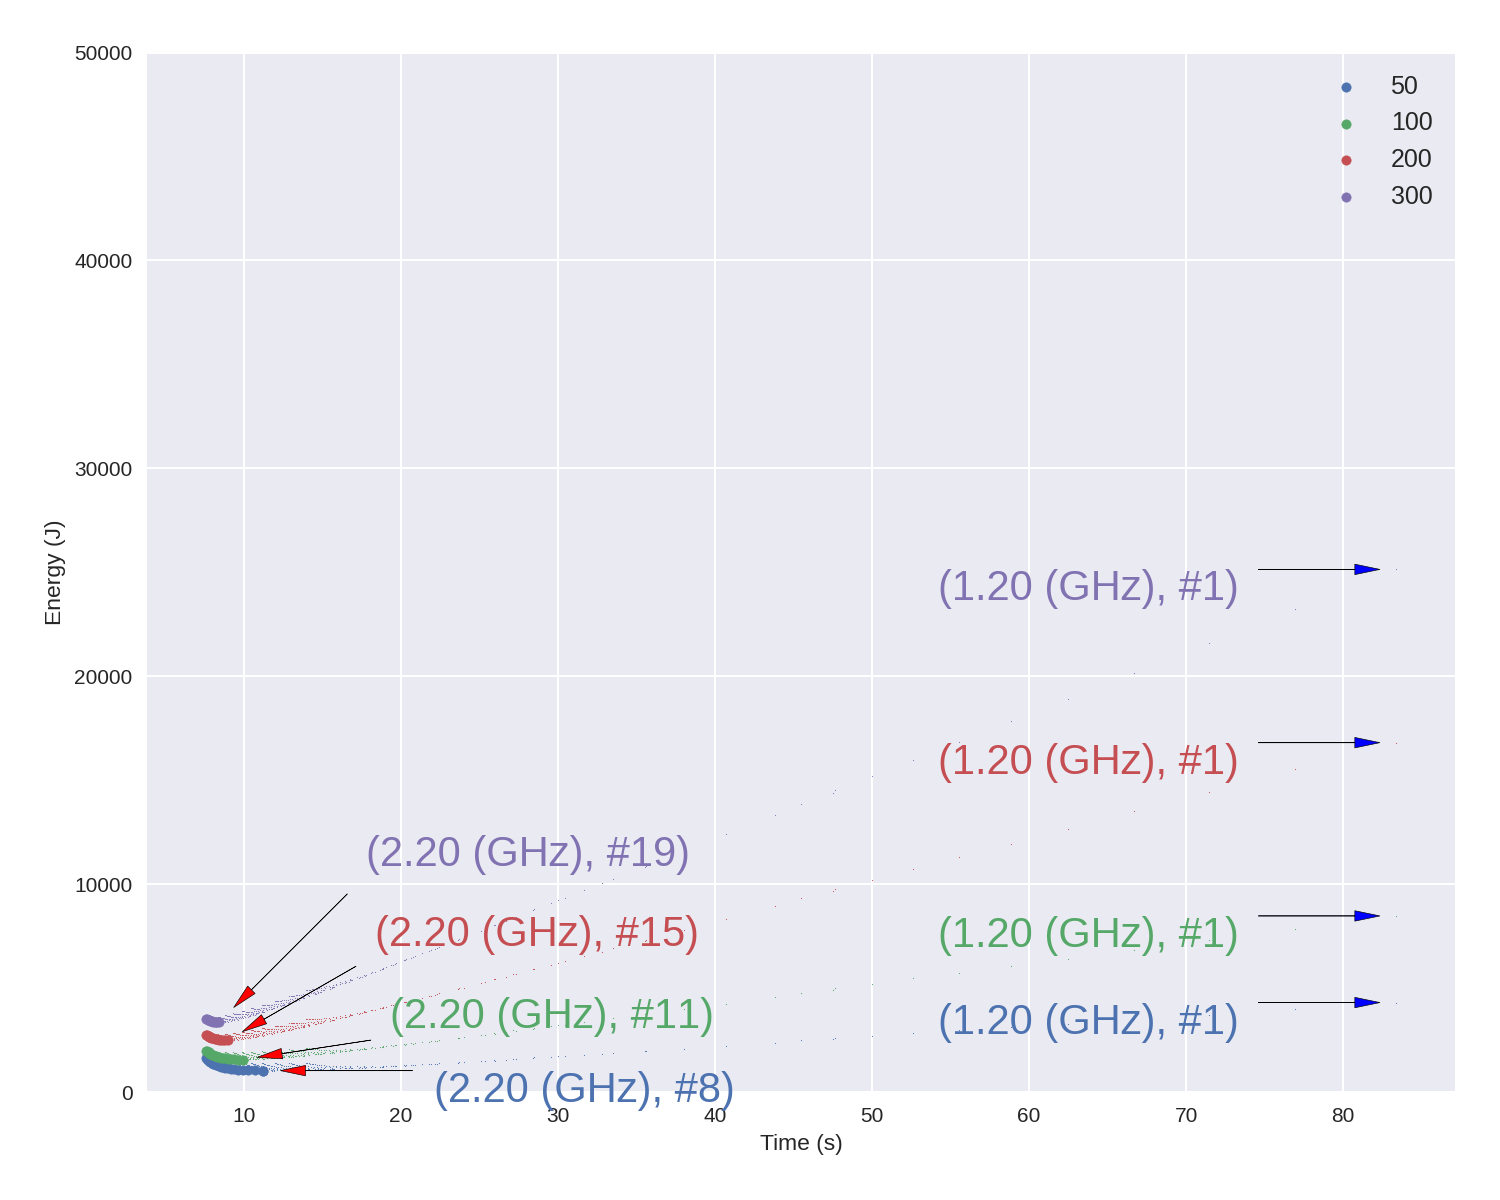
\includegraphics[width=\columnwidth]{analisys/pareto_static_low.png}
    \caption{Pareto w energy}
    \label{fig:pareto_w_l}
\end{figure}

\subsection{DVFS and DPM optimization} \label{sec:dvfs_optmin}
The effectiveness of the proposed approach during optimization was evaluated with a simple algorithm that finds the optimal frequency and number of active cores from the equation proposed. The results were then compared to the Linux default choices for power management.

% With \cref{eq:en_final}, it is possible to calculate energy consumption estimates for each possible configuration since there is a finite range of possible values for the frequency and number of cores. It is also possible to apply constraints on the execution time, frequency, and number of active cores. Then, the configuration that minimizes energy consumption for a given input can be selected. 

% Current HPC managers leave the user the choice of how many cores to use. On this basis, three situations were analyzed with relation to the number of cores:

% \begin{enumerate}
%     \item Worst choice: number of cores that maximize the total energy consumed;
%     \item Random choice: energy consumed for a random choice of number of cores;
%     \item Best choice: number of cores that minimize the total energy consumed (oracle).
% \end{enumerate}

% The default option for the Linux governor is Ondemand, and by default, it has no DPM control for the number of active cores. As Ondemand only does DVFS, for comparison, each application was executed with all available cores in the system, from 1 to 32.

% Figures \ref{fig:energy_worst_case}, \ref{fig:energy_mean_case}, and \ref{fig:energy_best_case}, show the energy savings with respect to Ondemand, i.e. $\frac{Ondemand-Model_{min}}{Ondemand}$ for the three cases described above. The savings and losses for each case are:
% \begin{enumerate}
%     \item Worst choice: save 69.88\% on average;
%     \item Random choice: save 12.04\% on average;
%     \item Best choice: lost 14.06\% on average.
% \end{enumerate}
% \begin{figure}[htb!]
%     \centering
%     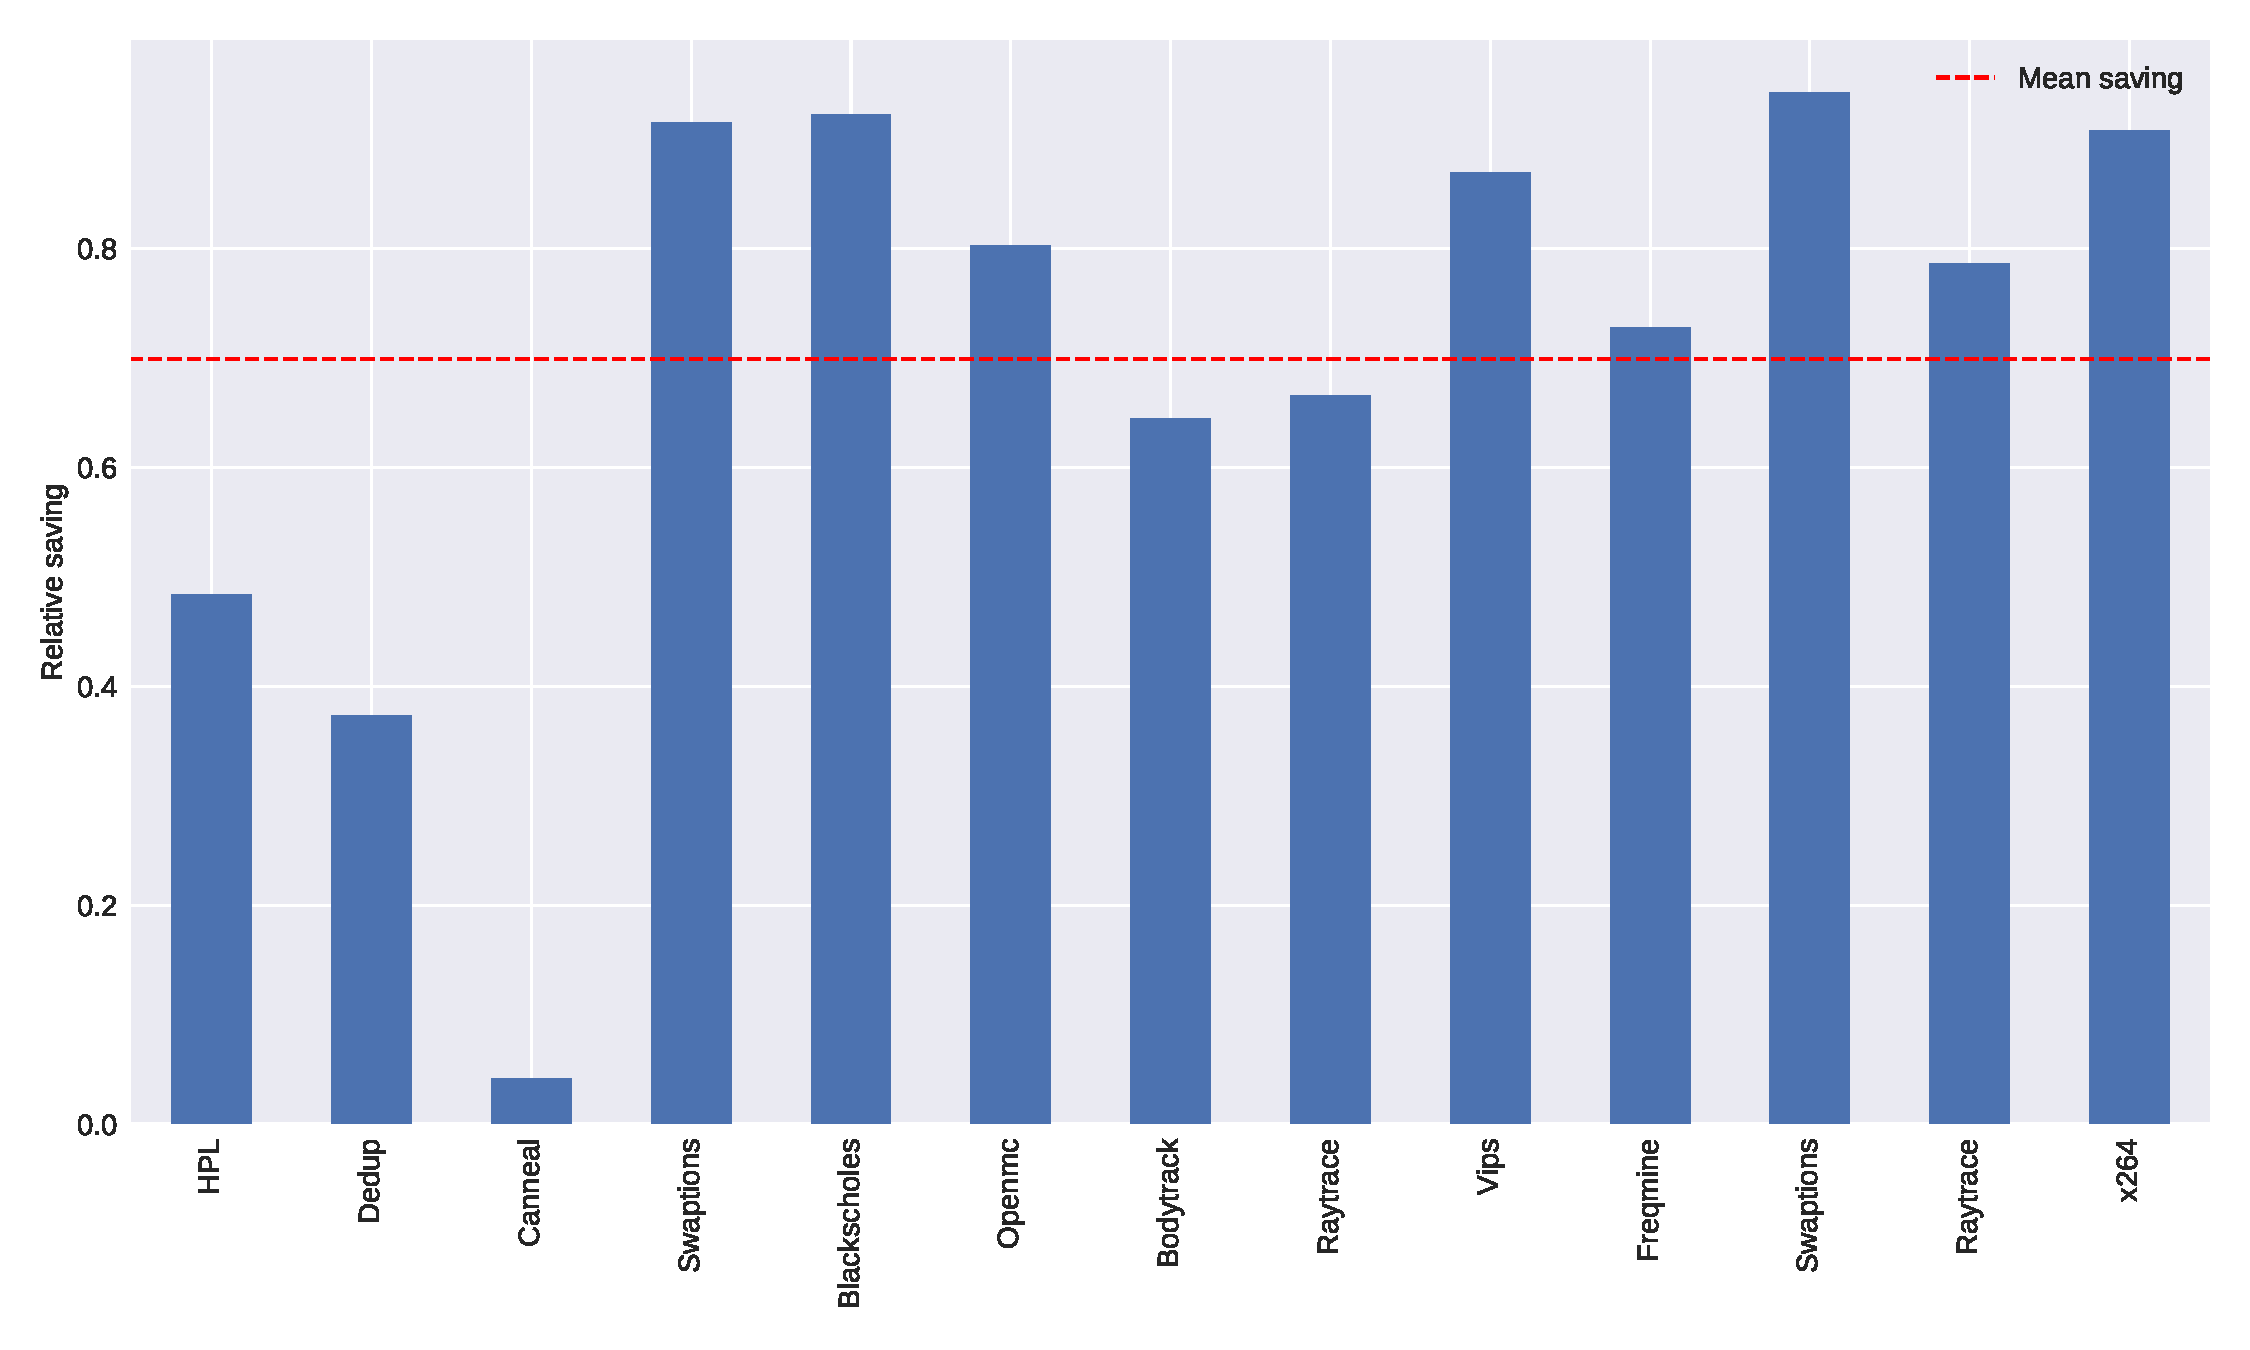
\includegraphics[width=\columnwidth]{dvfs_cmp_max.png}
%     \caption{Energy savings comparisons between the proposed model and the Worst case.}
%     \label{fig:energy_worst_case}
% \end{figure}
% \begin{figure}[htb!]
%     \centering
%     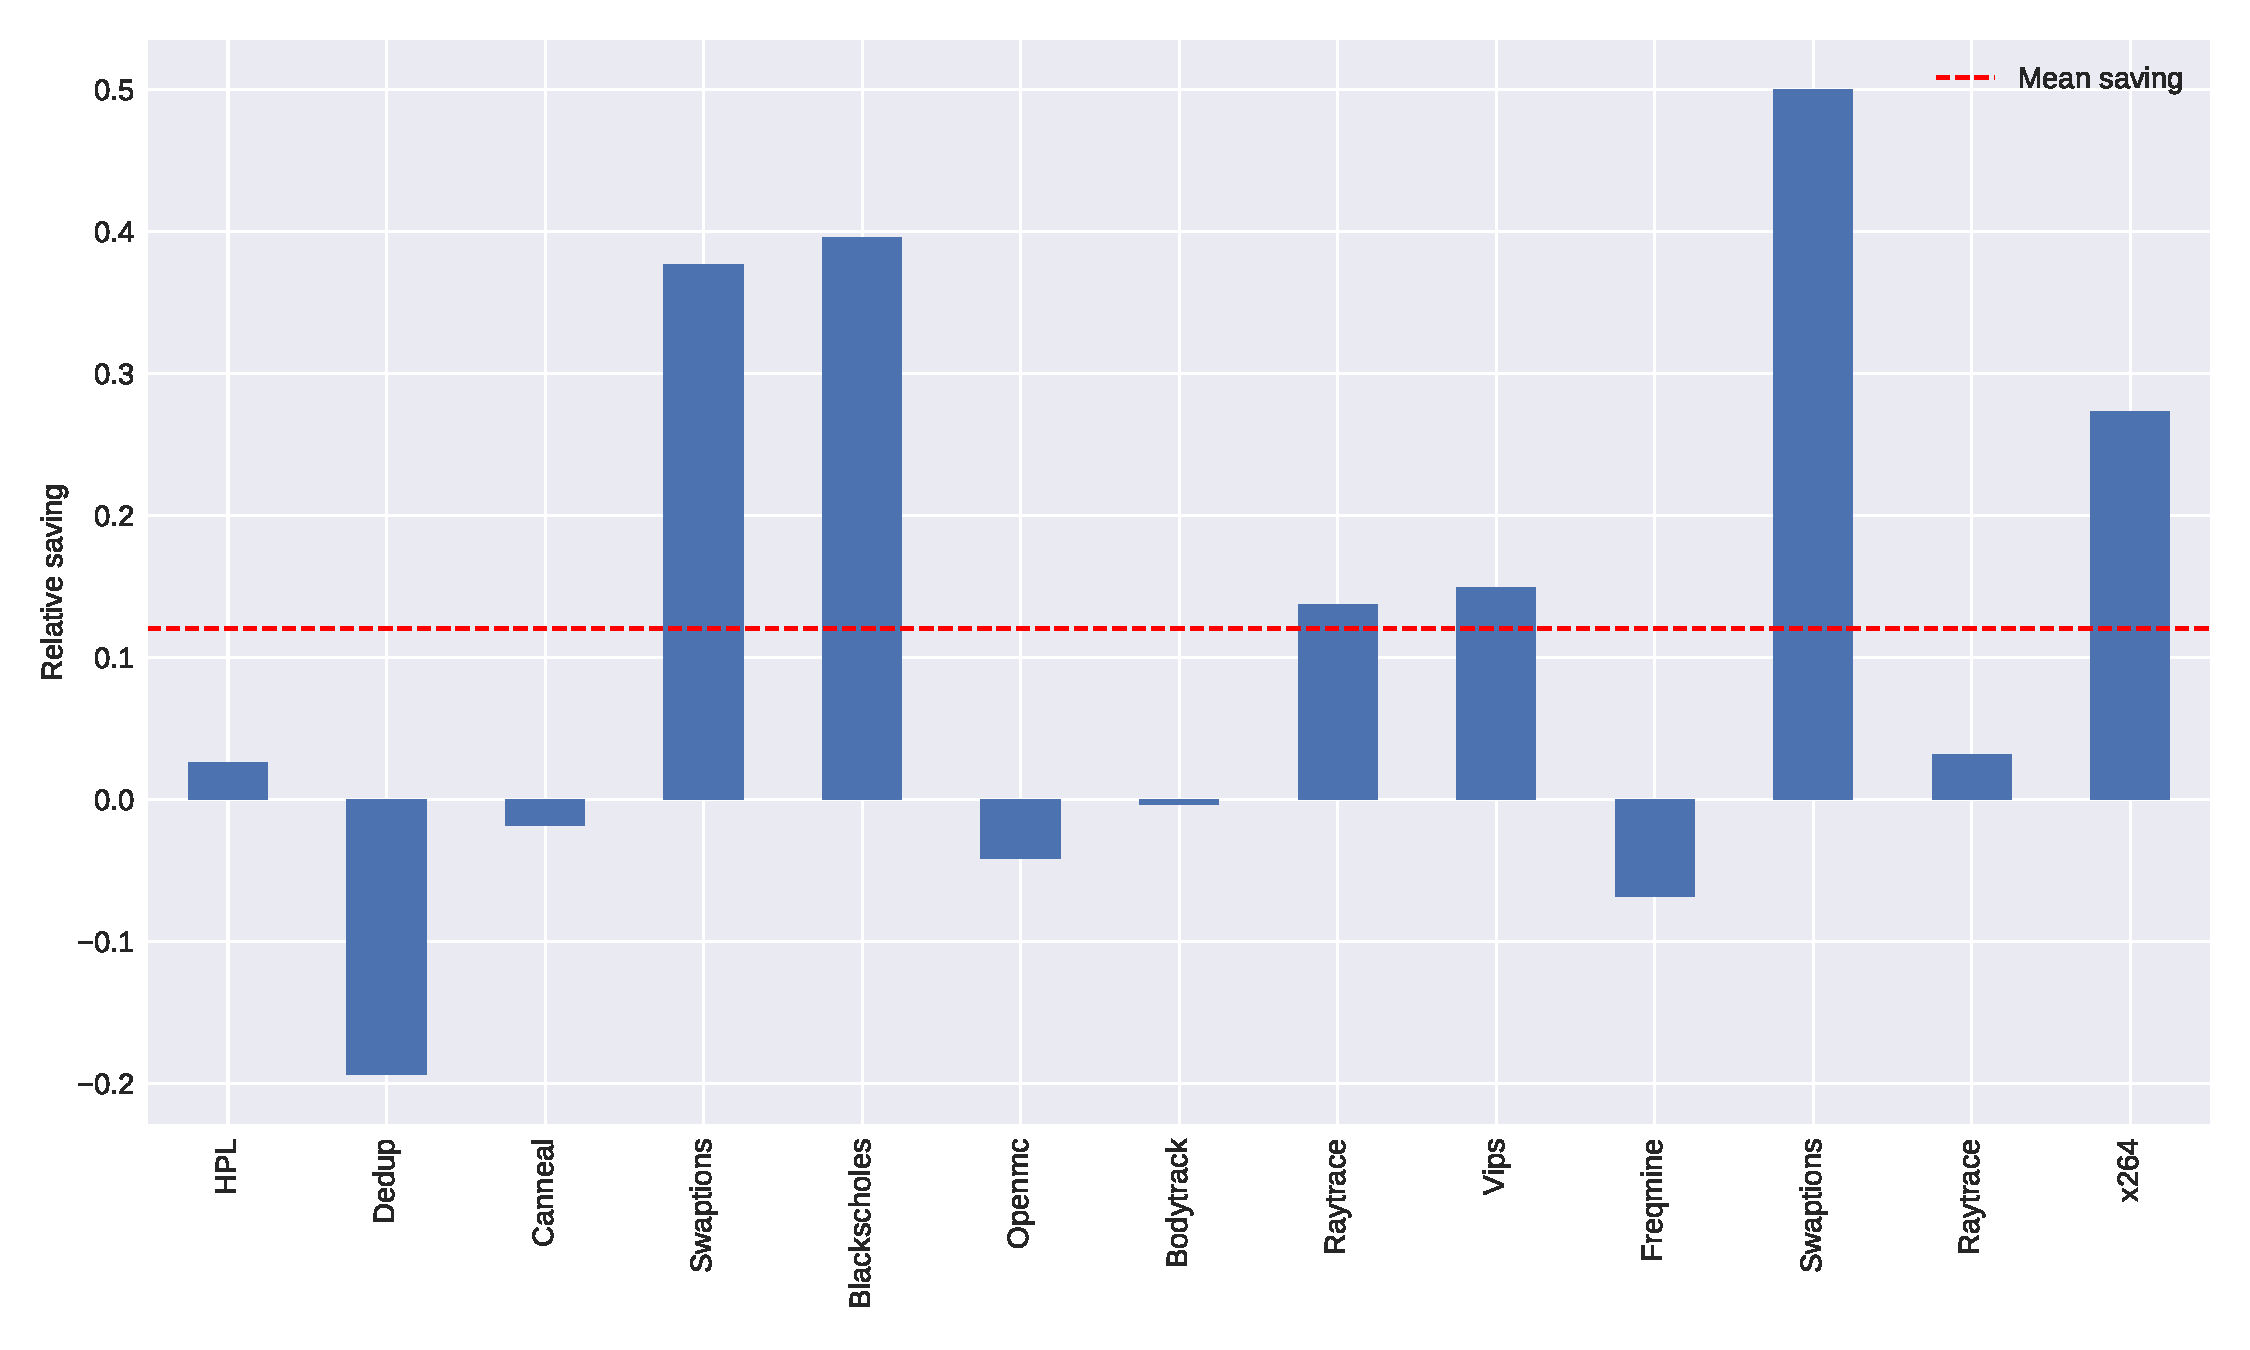
\includegraphics[width=\columnwidth]{dvfs_cmp_mean.png}
%     \caption{Energy savings comparisons between the proposed model and the Random case.}
%     \label{fig:energy_mean_case}
% \end{figure}
% \begin{figure}[htb!]
%     \centering
%     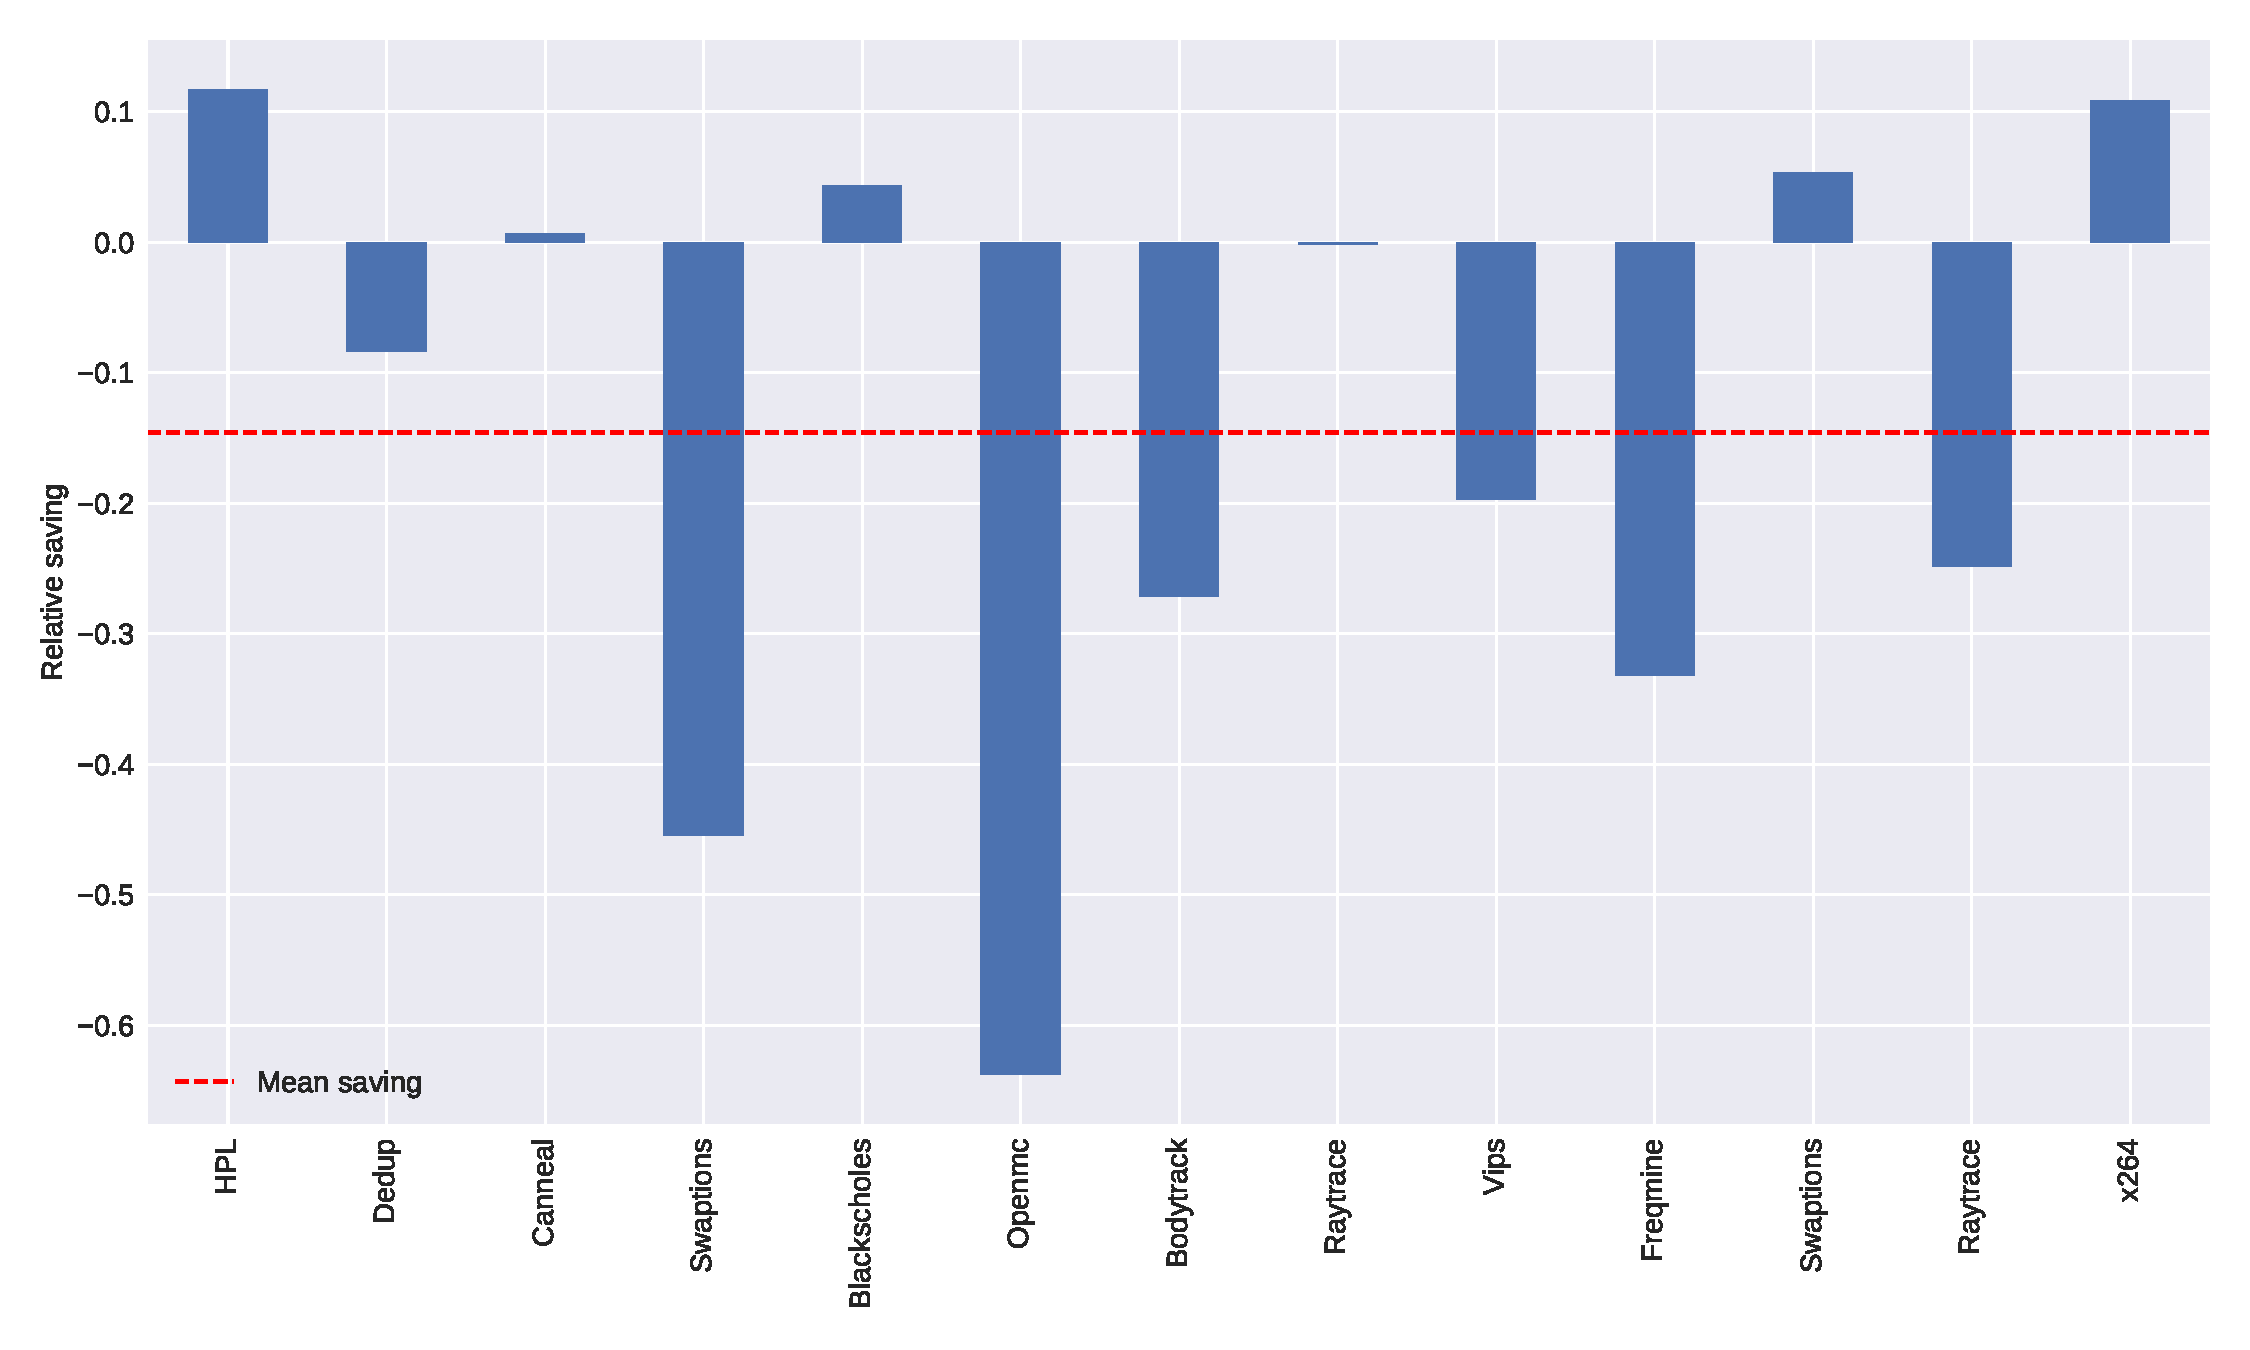
\includegraphics[width=\columnwidth]{dvfs_cmp_32.png}
%     \caption{Energy savings comparisons between the proposed model and the Best case.}
%     \label{fig:energy_best_case}
% \end{figure}

% By default, operating systems do not implement DPM at the core level, and in HPC the user usually explicitly chooses the number of cores to run their job. To give a better idea of the impact on the energy consumption of DPM at the core level, we analyzed the choices of the number of cores over a period of one year in the HPC center of the UFRN. The result is plotted in Figure \ref{fig:cpu_requests}.
% \begin{figure}[htb!]
%     \centering
%     \includegraphics[width=\columnwidth]{cpu_request.png}
%     \caption{Number of CPU requests during one year in HPC cluster, sorted by the number of cores requested per job.}
%     \label{fig:cpu_requests}
% \end{figure}

% Observe that the most common choice of many regular users is a single core requested per job, matching the worst case choice for all application analysed in this work. The best choice was quite often 32 cores, which is the third most popular choice among users, but it is 72 times less frequent than 1 core. This leads us to envision how much energy could be saved and encourage us towards future work using the proposed model for DPM or more advanced optimization algorithms.

% In practice, this approach can be brought into production by allowing the resource manager to perform these changes for the user using pre-scripts and post-scripts for high energy consumption job submissions.


\section{Conclusion} \label{sec:conclusion}
In this work we have proposed an energy model based on the operating frequency and the number of cores for a shared memory system. This model serves as a reference for DVFS and DPM optimization problems.

Results from 3 different HPC benchmarks demonstrate the potential of the proposed model. While consuming  10 times less energy than a machine learning approach, such as SVR, to characterize applications, it can be used to provide knowledgeable hints to improve DVFS and DPM algorithms by enabling analysis of the contribution of each model parameter (e.g. level of parallelism) to the energy consumption. Indeed, as shown in Section \ref{sec:dvfs_optmin}, when no oracle is available to choose the frequency and the number of cores the application should use, the proposed model can save around 12\% of energy for a random choice and up to 70\% for the worse possible choice. Considering the job history of our own HPC center which shows the prevalence of worse choices made by users, the potential energy savings are very significant and encourages further research.

Future work will demonstrate all possible analyzes achievable with the proposed equation as more advanced DVFS models can be derived from it. For instance, identifying the different phases of a target program will allow finer changes in frequency and, perhaps, in the number of active cores, to further improve the results presented here.

% \appendices
\section*{Acknowledgment}
We would like to acknowledge the use of UFRN´s High-Performance Computing Center (NPAD/UFRN), for running the experiments of this work, and thank NPAD´s team for providing the necessary support to perform the energy measurements. 
% \footnote{NPAD is the name of the High Performance Computing Center (from Portuguese: Núcleo de Processamento de Alto Desempenho) of the Universidade Federal do Rio Grande do Norte (UFRN)}.



\bibliographystyle{IEEEtran}
\bibliography{references.bib}

%\bibliographystyle{IEEEtran}
%\begin{thebibliography}{00}
%\bibliography{references}
%\end{thebibliography}

\section*{Appendix}

The following abbreviations are used in this manuscript:\\

\noindent 
\begin{tabular}{@{}ll}
DVFS Dynamic Frequency and Voltage Scaling\\
DPM Dynamic Power Management\\
SVR Support Vector Regression\\
RBF Radial Base Function\\
HPC High Performance Computing\\
IPMI The Intelligent Platform Management Interface\\
RBF Radial Base Function\\
MPE Mean Percentage Error
\end{tabular}


\begin{IEEEbiography}[{\includegraphics[width=1in,height=1.25in,clip,keepaspectratio]{./figures/biography_vitorramos}}]{Vitor R. G. Silva}
Bsc in Science and Technology in 2016 and Computer Engineer in 2018 by Federal University of Rio Grande do Norte. His research interests are high-performance computing, operating systems, cybersecurity and Artificial intelligence.
\end{IEEEbiography}

\begin{IEEEbiography}[{\includegraphics[width=1in,height=1.25in,clip,keepaspectratio]{./figures/biography_carlos}}]{Carlos A. V. Sakuyama}
Professor Valderrama is, since 2004, Director of the Electronics and Microelectronics Department at the Polytechnic Faculty of the University of Mons in Belgium.  His Department is member of the New Media Art Technology and the Information Technology Institutes. He obtained the Ph.D. degree in Microelectronics at the Institute Nationale Polytechnique de Grenoble INPG (today Grenoble Institute of Technology) at the TIMA lab in France, in 1998, the M.Sc. diploma at the Federal University of Rio de Janeiro, Brazil, in 1993, and the electrical-electronics engineering diploma at the National University of Cordoba, Argentina, in 1989. He was invited professor in several universities, the Catholic University of Cordoba (Argentina), the Federal University of Pernambuco and the Federal University of Rio Grande do Norte (Brazil) and the University of Castilla La Mancha (Spain). He was responsible for the creation of the spinoff Nsilition (2009, funded by the Walloon Region). He has participated in more than 18 national and international research projects from the development of 4G chips, tracking devices and architectures for IoT, HPC and space.  He serves as technical reviewer and committee member of multiple journals and international conferences. His research activity is supported by more than 180 publications on international conferences, more than 10 books chapters, and more than 30 scientific journals. He is IEEE senior member since 2006.
\end{IEEEbiography}

\begin{IEEEbiography}[{\includegraphics[width=1in,height=1.25in,clip,keepaspectratio]{./figures/samuel}}]{Samuel Xavier-de-Souza}
SAMUEL XAVIER-DE-SOUZA (Senior Member, IEEE) was born in Natal, Brazil. He received the Computer Engineering degree from the Universidade Federal do Rio Grande do Norte-UFRN, Brazil, in 2000, and the Ph.D. degree in electrical engineering from Katholieke Universiteit Leuven, Belgium, in 2007. He worked for IMEC, Belgium, as a Software/Hardware Engineer, and for the Flemish Supercomputing Center, Belgium, as a High-Performance Computing Consultant. In 2009, he joined the Department of Computer Engineering and Automation of UFRN, where he currently holds the position of an Associate Professor. He is also a Founder and the Director of UFRN’s High-Performance Computing Center-NPAD. In 2016, he became a Royal Society-Newton Advanced Fellow. His research interests include software energy, scalable and efficient parallel systems, parallel algorithms, parallel architectures, and their applications.
\end{IEEEbiography}

\EOD

\end{document}

